\subsection{WEIGHTS OF A FINITE DIMENSIONAL SIMPLE g-MODULE}

PROPOSITION 1. Let V be a finite dimensional g-module.

\begin{enumerate}
\def\labelenumi{(\roman{enumi})}
\item
  All the weights of V belong to P.
\item
  \(V = \bigoplus_{\mu \in P} V^{\mu}.\)
\item
  For all \(\mu \in \mathfrak{h}^*\) , \(\mathrm{V}^{\mu}\) is the set of \(x \in \mathrm{V}\) such that \(h.x = \mu(h)x\) for all \(h \in \mathfrak{h}\) .
\end{enumerate}

For all \(\alpha \in \mathrm{B}\) , there exists a homomorphism from \(\mathfrak{sl}(2,k)\) to \(\mathfrak{g}\) that takes \(H\) to \(H_{\alpha}\) . Thus, by §1, no. 2, Cor. of Prop. 2, \((H_{\alpha})_{\mathrm{V}}\) is diagonalizable and its eigenvalues are integers. Hence, the set of \((H_{\alpha})_{\mathrm{V}}\) , for \(\alpha \in \mathrm{B}\) , is diagonalizable (Algebra, Chap. VII, §5, no. 6, Prop. 13). Consequently, for all \(h \in \mathfrak{h}\) , \(h_{\mathrm{V}}\) is diagonalizable. By Chap. VII, §1, no. 3, Prop. 9, \(\mathrm{V} = \bigoplus_{\mu \in \mathfrak{h}^*} \mathrm{V}^{\mu}\) . On the other hand, if \(\mathrm{V}^{\mu} \neq 0\) , the preceding shows that \(\mu(H_{\alpha}) \in \mathbf{Z}\) for all \(\alpha \in \mathrm{B}\) , so \(\mu \in \mathrm{P}\) . This proves (i) and (ii). We see in the same way that \(\mathfrak{h}_{\mathrm{V}}\) is diagonalizable, hence (iii).

COROLLARY. Let \(\rho\) be a finite dimensional representation of \(\mathfrak{g}\) and \(\Phi\) the bilinear form associated to \(\rho\) .

\begin{enumerate}
\def\labelenumi{(\roman{enumi})}
\item
  If \(x, y \in \mathfrak{h}_{\mathbf{Q}}\) , then \(\Phi(x, y) \in \mathbf{Q}\) and \(\Phi(x, x) \in \mathbf{Q}_{+}\) .
\item
  If \(\rho\) is injective, the restriction of \(\Phi\) to \(\mathfrak{h}\) is non-degenerate.
\end{enumerate}

Assertion (i) follows from Prop. 1 since the elements of P have rational values on \(\mathfrak{h}_{\mathbf{Q}}\) . If \(\rho\) is injective, \(\Phi\) is non-degenerate (Chap. I, §6, no. 1, Prop. 1), so the restriction of \(\Phi\) to \(\mathfrak{h}\) is non-degenerate (Chap. VII, §1, no. 3, Prop. 10 (iii)).

Lemma 1. Let \(\mathrm{V}\) be a \(\mathfrak{g}\) -module and \(\rho\) the corresponding representation of \(\mathfrak{g}\) .

\begin{enumerate}
\def\labelenumi{(\roman{enumi})}
\tightlist
\item
  If \(a\) is a nilpotent element of \(\mathfrak{g}\) , and if \(\rho(a)\) is locally nilpotent,
\end{enumerate}

\[
\rho (e ^ {\mathrm{ad} a} b) = e ^ {\rho (a)} \rho (b) e ^ {- \rho (a)}
\]

for all \(b \in \mathfrak{g}\).

\begin{enumerate}
\def\labelenumi{(\roman{enumi})}
\setcounter{enumi}{1}
\tightlist
\item
  If \(\alpha \in \mathrm{R}\) and if the images under \(\rho\) of the elements of \(\mathfrak{g}^{\alpha}\) and \(\mathfrak{g}^{-\alpha}\) are locally nilpotent, the set of weights of \(V\) is stable under the reflection \(s_{\alpha}\) .
\end{enumerate}

With the assumptions in (i), we have \(\rho((\mathrm{ad}a)^n b) = (\mathrm{ad}\rho(a))^n\rho(b)\) for all \(n\geq 0\) , so \(\rho(e^{\mathrm{ad}a}b) = e^{\mathrm{ad}\rho(a)}\rho(b)\) . On the other hand,

\[
e ^ {\mathrm{ad} \rho (a)} \rho (b) = e ^ {\rho (a)} \rho (b) e ^ {- \rho (a)}
\]

is assertion (ii) of Chap. VII, §3, no. 1, Lemma 1.

We now adopt the assumptions in (ii). Let \(\theta_{\alpha} = e^{\mathrm{ad}X_{\alpha}}e^{\mathrm{ad}X_{-\alpha}}e^{\mathrm{ad}X_{\alpha}}\) . By (i), there exists \(S\in \mathbf{GL}(V)\) such that \(\rho (\theta_{\alpha}b) = S\rho (b)S^{-1}\) for all \(b\in \mathfrak{g}\) . Now \(\theta_{\alpha}|\mathfrak{h}\) is the transpose of \(s_{\alpha}\) (§2, no. 2, Lemma 1). Let \(\lambda\) be a weight of V. There exists a non-zero element \(x\) of V such that \(\rho (h)x = \lambda (h)x\) for all \(h\in \mathfrak{h}\) . Then

\[
\rho (h) \mathrm{S} ^ {- 1} x = \mathrm{S} ^ {- 1} \rho (^ {t} s _ {\alpha} h) x = \mathrm{S} ^ {- 1} \lambda (^ {t} s _ {\alpha} h) x = (s _ {\alpha} \lambda) (h) \mathrm{S} ^ {- 1} x
\]

for all \(h \in \mathfrak{h}\) . Consequently, \(s_{\alpha}\lambda\) is a weight of V.

PROPOSITION 2. Let \(\mathrm{V}\) be a finite dimensional \(\mathfrak{g}\) -module and \(s \in \operatorname{Aut}_0(\mathfrak{g})\) .

\begin{enumerate}
\def\labelenumi{(\roman{enumi})}
\item
  There exists \(\mathrm{S} \in \mathbf{GL}(\mathrm{V})\) such that \((s(x))_{\mathrm{V}} = \mathrm{S}x_{\mathrm{V}}\mathrm{S}^{-1}\) for all \(x \in \mathfrak{g}\) .
\item
  If \(s \in \mathrm{Aut}_e(\mathfrak{g})\) , \(S\) can be chosen to be an element of \(\mathbf{SL}(V)\) leaving stable all the \(\mathfrak{g}\) -submodules of \(V\) .
\end{enumerate}

Assertion (ii) follows from Lemma 1 (i). Now let \(s \in \mathrm{Aut}_0(\mathfrak{g})\) and denote by \(\rho\) the representation of \(\mathfrak{g}\) defined by V. By (ii), the representations \(\rho\) and \(\rho \circ s\) become equivalent after extension of scalars. They are therefore equivalent (Chap. I, §3, no. 8, Prop. 13), hence the existence of S.

Remark 1. Let S satisfy the condition in Prop. 2 (i), and let \(\mathfrak{h}' = s(\mathfrak{h})\) ; denote by \(s^*\) the isomorphism \(\lambda \mapsto \lambda \circ s^{-1}\) from \(\mathfrak{h}^*\) to \(\mathfrak{h}'^*\) . It is clear that

\[
\mathrm{S} (\mathrm{V} ^ {\lambda}) = \mathrm{V} ^ {s ^ {*} \lambda}.
\]

In particular:

COROLLARY 1. The isomorphism \(s^*\) takes the weights of V with respect to \(\mathfrak{h}\) to those of V with respect to \(\mathfrak{h}'\) ; corresponding weights have the same multiplicity.

COROLLARY 2. Let \(w \in \mathrm{W}\) . For all \(\lambda \in \mathfrak{h}^*\) , the vector subspaces \(\mathrm{V}^{\lambda}\) and \(\mathrm{V}^{w\lambda}\) have the same dimension. The set of weights of \(\mathrm{V}\) is stable under \(\mathrm{W}\) .

Indeed, \(w\) is of the form \(s^*\) with \(s \in \mathrm{Aut}_e(\mathfrak{g}, \mathfrak{h})\) (§2, no. 2, Cor. of Th. 2).

Remark 2. By Cor. 1 of Prop. 2 and §5, no. 3, Remark 2, it makes sense to speak of the weights of V with respect to the canonical Cartan subalgebra of g, and of their multiplicities.

Remark 3. Lemma 1 (i) and Prop. 2 remain valid, with the same proof, even if g is not assumed to be splittable.

\subsection{HIGHEST WEIGHT OF A FINITE DIMENSIONAL SIMPLE g-MODULE}

THEOREM 1. A simple g-module is finite dimensional if and only if it has a highest weight belonging to \(P_{++}\) .

We denote by V a simple g-module and by X its set of weights.

\begin{enumerate}
\def\labelenumi{\alph{enumi})}
\item
  Assume that V is finite dimensional. Then X is finite and non-empty (Prop. 1) and so has a maximal element \(\omega\) . Let \(\alpha \in B\) . Then \(\omega + \alpha \notin X\) , which proves that \(\omega\) is the highest weight of V (§6, no. 2, Lemma 2). On the other hand, there exists a homomorphism from \(\mathfrak{sl}(2, k)\) to g that takes H to \(H_{\alpha}\) ; by §1, Prop. 2 (i), \(\omega(H_{\alpha})\) is an integer \(\geq 0\) , so \(\omega \in P_{++}\) .
\item
  Assume that V has a highest weight \(\omega\in P_{++}\) . Let \(\alpha\in B\) and let e be a primitive element of weight \(\omega\) in V. Put \(e_{j}=X_{-\alpha}^{j}e\) for \(j\geq0\) , \(m=\omega(H_{\alpha})\in N\) , and \(N=\sum_{j=0}^{m}ke_{j}\) . By §1, no. 2, Prop. 1, \(X_{\alpha}e_{m+1}=0\) . If \(\beta\in B\) and \(\beta\neq\alpha\) , then \([X_{\beta},X_{-\alpha}]=0\) so \(X_{\beta}e_{m+1}=X_{\beta}X_{-\alpha}^{m+1}e=X_{-\alpha}^{m+1}X_{\beta}e=0\) . If \(e_{m+1}\neq0\) , we conclude that \(e_{m+1}\) is primitive, which is absurd (§6, Prop. 3 (i)); so \(e_{m+1}=0\) . Thus, by §1, no. 2, Cor. of Prop. 1, N is stable under the subalgebra \(s_{\alpha}\) generated by \(H_{\alpha},X_{\alpha}\) and \(X_{-\alpha}\) . Now \(s_{\alpha}\) is reductive in g, so the sum of the finite dimensional subspaces of V that are stable under \(s_{\alpha}\) is a g-submodule of V (Chap. I, §6, no. 6, Prop. 7); since this sum is non-zero, it is equal to V. It follows from this that \((X_{\alpha})_{V}\) and \((X_{-\alpha})_{V}\) are locally nilpotent. In view of Lemma 1 (ii), X is stable under \(s_{\alpha}\) , and this holds for all \(\alpha\) . Hence X is stable under W. Now every orbit of W on P meets \(P_{++}\) (Chap. VI, §1, no. 10). On the other hand, if \(\lambda\in X\cap P_{++}\) , then \(\lambda=\omega-\sum_{\alpha\in B}n_{\alpha}\alpha=\sum_{\alpha\in B}n'_{\alpha}\alpha\) with \(n_{\alpha}\in N\) and \(n'_{\alpha}\geq0\) for all \(\alpha\in B\) (Chap. V, §3, no. 5, Lemma 6). So \(X\cap P_{++}\) is finite and hence so is X. Since each weight has finite multiplicity (§6, no. 1, Prop. 1 (ii)), V is finite dimensional.
\end{enumerate}

COROLLARY 1. If \(\lambda \in \mathfrak{h}^*\) and \(\lambda \notin \mathrm{P}_{++}\) , the \(\mathfrak{g}\) -module \(\mathrm{E}(\lambda)\) (§6, no. 3) is infinite dimensional.

COROLLARY 2. The g-modules \(E(\lambda)\) for \(\lambda \in P_{++}\) constitute a set of representatives of the classes of finite dimensional simple g-modules.

The g-modules \(E(\lambda)\) , where \(\lambda\) is a fundamental weight, are called the fundamental g-modules; the corresponding representations are called the fundamental representations of g; they are absolutely irreducible ( \(\S6\) , no. 2, Prop. 3 (iv)).

If V is a finite dimensional g-module and \(\lambda\in P_{++}\) , the isotypical component of V of type \(\mathrm{E}(\lambda)\) is called the isotypical component of highest weight \(\lambda\) of V.

Remark 1. Let \(\lambda \in \mathrm{P}_{++}\) , \(\rho_{\lambda}\) the representation of \(\mathfrak{g}\) on \(\operatorname{E}(\lambda)\) , \(s \in \operatorname{Aut}(\mathfrak{g})\) , and \(\sigma\) the canonical image of \(s\) in \(\operatorname{Aut}(\mathrm{R},\mathrm{B})\) ( \(\S 5\) , no. 3, Cor. 1 of Prop. 5). Then \(\rho_{\lambda} \circ s\) is equivalent to \(\rho_{\sigma \lambda}\) ; indeed, if \(s \in \operatorname{Aut}_0(\mathfrak{g})\) , \(\rho_{\lambda} \circ s\) and \(\rho_{\sigma \lambda}\) are equivalent to \(\rho_{\lambda}\) (Prop. 2); and, if \(s\) leaves \(\mathfrak{h}\) and B stable, \(\rho_{\lambda} \circ s\) is simple of highest weight \(\sigma \lambda\) .

In particular, the fundamental representations are permuted by \(s\) , and this permutation is the identity if and only if \(s \in \mathrm{Aut}_0(\mathfrak{g})\) .

PROPOSITION 3. Let V be a finite dimensional g-module and X its set of weights. Let \(\lambda \in X\) , \(\alpha \in R\) , I the set of \(t \in Z\) such that \(\lambda + t\alpha \in X\) , p (resp. -q) the largest (resp. smallest) element of I. Let \(m_t\) be the multiplicity of \(\lambda + t\alpha\) .

\begin{enumerate}
\def\labelenumi{(\roman{enumi})}
\item
  I = \(\{-q, p\}\) and \(q - p = \lambda(H_{\alpha})\) .
\item
  For any integer \(u \in [0, p + q]\) , \(\lambda + (p - u)\alpha\) and \(\lambda + (-q + u)\alpha\) are conjugate under \(s_{\alpha}\) , and \(m_{-q + u} = m_{p - u}\) .
\item
  If \(t \in \mathbf{Z}\) and \(t < (p - q)/2\) , \((X_{\alpha})_{\mathrm{V}}\) maps \(V^{\lambda + t\alpha}\) injectively into \(V^{\lambda + (t + 1)\alpha}\) .
\item
  The function \(t \mapsto m_t\) is increasing on \([-q, (p - q)/2]\) and decreasing on \([(p - q)/2, p]\) .
\end{enumerate}

Let \(\alpha \in \mathrm{B}\) . Give V the \(\mathfrak{sl}(2,k)\) -module structure defined by the elements \(X_{\alpha}, X_{-\alpha}, H_{\alpha}\) of \(\mathfrak{g}\) . Every non-zero element of \(\mathrm{V}^{\lambda + p\alpha}\) is then primitive. Consequently, \((\lambda + p\alpha)(H_{\alpha}) \geq 0\) and \((X_{-\alpha})^{r}\mathrm{V}^{\lambda + p\alpha} \neq 0\) for

\[
0 \leq r \leq (\lambda + p \alpha) (H _ {\alpha}) = \lambda (H _ {\alpha}) + 2 p
\]

\pandocbounded{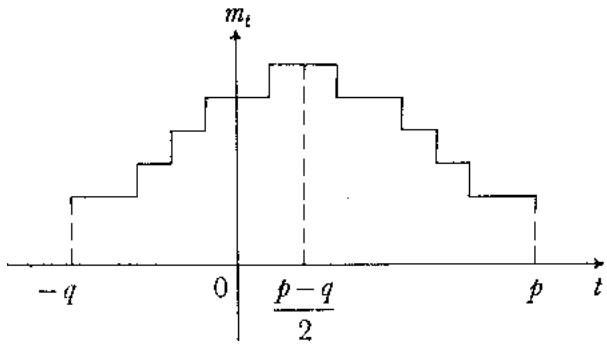
\includegraphics[keepaspectratio]{images/part001_39d2730e.jpg}}

(§1, no. 2, Prop. 2). It follows that \(\mathrm{V}^{\lambda + t\alpha} \neq 0\) for \(p \geq t \geq p - (\lambda(H_{\alpha}) + 2p)\) , so \(p + q \geq \lambda(H_{\alpha}) + 2p\) . Applying this result to \(-\alpha\) gives

\[
p + q \geq \lambda (H _ {- \alpha}) + 2 q = - \lambda (H _ {\alpha}) + 2 q.
\]

Hence \(q - p = \lambda (H_{\alpha})\) and \(\lambda + t\alpha \in \mathcal{X}\) for \(p \geq t \geq -q\) , which proves (i).

We have \(s_{\alpha}(\alpha) = -\alpha\) , and \(s_{\alpha}(\mu) \in \mu + k\alpha\) for all \(\mu \in \mathfrak{h}^*\) . Since W leaves \(\mathcal{X}\) stable (Cor. 2 of Prop. 2), \(s_{\alpha}\) leaves \(\{\lambda - q\alpha, \lambda - q\alpha + \alpha, \ldots, \lambda + p\alpha\}\) stable and takes \(\lambda - q\alpha + u\alpha\) to \(\lambda + p\alpha - u\alpha\) for all \(u \in k\) . Using Cor. 2 of Prop. 2 again, we see that \(m_{-q + u} = m_{p - u}\) for every integer \(u \in [0, p + q]\) . This proves (ii).

By §1, Cor. of Prop. 2, \((X_{\alpha})_{\mathrm{V}}|\mathrm{V}^{\lambda +t\alpha}\) is injective for \(t < (p - q) / 2\) . Now \((X_{\alpha})_{\mathrm{V}}\) maps \(\mathrm{V}^{\lambda +t\alpha}\) to \(\mathrm{V}^{\lambda +(t + 1)\alpha}\) . Hence \(m_{t + 1}\geq m_t\) for \(t < (p - q) / 2\) . Changing \(\alpha\) to \(-\alpha\) , we see that \(m_{t + 1}\leq m_t\) for \(t > (p - q) / 2\) . This proves (iii) and (iv).

COROLLARY 1. If \(\lambda \in \mathcal{X}\) and \(\lambda (H_{\alpha})\geq 1\) , then \(\lambda -\alpha \in \mathcal{X}\) . If \(\lambda +\alpha \in \mathcal{X}\) and \(\lambda (H_{\alpha}) = 0\) , then \(\lambda \in \mathcal{X}\) and \(\lambda -\alpha \in \mathcal{X}\) .

This follows immediately from Prop. 3 (i).

COROLLARY 2. Let \(\mu \in \mathrm{P}_{++}\) and \(\nu \in \mathrm{Q}_{+}\) . If \(\mu + \nu \in \mathcal{X}\) , then \(\mu \in \mathcal{X}\) .

Write \(\nu = \sum_{\alpha \in \mathrm{B}} c_{\alpha}.\alpha\) , where \(c_{\alpha} \in \mathbf{N}\) for all \(\alpha \in \mathrm{B}\) . The corollary is clear when \(\sum_{\alpha \in \mathrm{B}} c_{\alpha} = 0\) ; assume that \(\sum_{\alpha \in \mathrm{B}} c_{\alpha} > 0\) and argue by induction on \(\sum_{\alpha \in \mathrm{B}} c_{\alpha}\) . Let \((\cdot|\cdot)\) be a W-invariant non-degenerate positive symmetric bilinear form on \(\mathfrak{h}_{\mathbf{R}}^{*}\) . Then \((\nu|\sum_{\alpha \in \mathrm{B}} c_{\alpha}.\alpha) > 0\) , so there exists \(\beta \in \mathrm{B}\) such that \(c_{\beta} \geq 1\) and \((\nu|\beta) > 0\) , hence \(\nu(H_{\beta}) \geq 1\) . Since \(\mu \in \mathrm{P}_{++}\) , it follows that \((\mu + \nu)(H_{\beta}) \geq 1\) . By Cor. 1, \(\mu + (\nu - \beta) \in \mathcal{X}\) , and it suffices to apply the induction hypothesis.

COROLLARY 3. Let \(v \in V\) be primitive of weight \(\omega\) . Let \(\Sigma\) be the set of \(\alpha \in B\) such that \(\omega(H_{\alpha}) = 0\) . The stabilizer in \(\mathfrak{g}\) of the line \(kv\) is the parabolic subalgebra \(\mathfrak{p}_{\Sigma}\) associated to \(\Sigma\) (§3, no. 4, Remark).

Replacing V by the g-submodule generated by v, if necessary, we can assume that V is simple. Let s be the stabilizer. We have \((\mathfrak{n}_{+})_{\mathrm{V}}v = 0\) , \((\mathfrak{h})_{\mathrm{V}}v \subset kv\) . Let \(\alpha \in B\) be such that \(\omega(H_{\alpha}) = 0\) . We have \(\omega + \alpha \notin X\) , hence \(\omega - \alpha \notin X\) (Prop. 3 (i)) and consequently \((\mathfrak{g}^{-\alpha})_{\mathrm{V}}v = 0\) . The preceding proves that \(p_{\Sigma} \subset s\) . If \(p_{\Sigma} \neq s\) , then \(s = p_{\Sigma'}\) , where \(\Sigma'\) is a subset of B strictly containing \(\Sigma\) . Let \(\beta \in \Sigma' - \Sigma\) . Then \(g^{-\beta}\) stabilizes kv, and hence annihilates v. But, since \(\omega(H_{\beta}) > 0\) , this contradicts Prop. 3 (iii). Q.E.D.

A subset \(\mathcal{X}\) of P is called R-saturated if it satisfies the following condition: for all \(\lambda \in \mathcal{X}\) and all \(\alpha \in \mathrm{R}\) , we have \(\lambda - t\alpha \in \mathcal{X}\) for all integers \(t\) between 0 and \(\lambda(H_{\alpha})\) . Since \(s_{\alpha}(\lambda) = \lambda - \lambda(H_{\alpha})\alpha\) , we see that an R-saturated subset of P is stable under W. Let \(\mathcal{Y} \subset \mathrm{P}\) . An element \(\lambda\) of \(\mathcal{Y}\) is called R-extremal in \(\mathcal{Y}\) if, for all \(\alpha \in \mathrm{R}\) , either \(\lambda + \alpha \notin \mathcal{Y}\) or \(\lambda - \alpha \notin \mathcal{Y}\) .

PROPOSITION 4. Let \(\mathrm{V}\) be a finite dimensional \(\mathfrak{g}\) -module and \(d\) an integer \(\geq 1\) . The set of weights of \(\mathrm{V}\) of multiplicity \(\geq d\) is R-saturated.

This follows immediately from Prop. 3.

PROPOSITION 5. Let V be a finite dimensional simple g-module, \(\omega\) its highest weight, X its set of weights. Choose a W-invariant non-degenerate positive symmetric bilinear form \((\cdot|\cdot)\) on \(h_{R}^{*}\) , and let \(\lambda\mapsto\|\lambda\|=(\lambda|\lambda)^{1/2}\) be the corresponding norm.

\begin{enumerate}
\def\labelenumi{(\roman{enumi})}
\item
  \(\mathcal{X}\) is the smallest R-saturated subset of P containing \(\omega\) .
\item
  The R-extremal elements of \(\mathcal{X}\) are the W-transforms of \(\omega\) .
\item
  If \(\mu \in \mathcal{X}\) , we have \(\| \mu \| \leq \| \omega \|\) . If, in addition, \(\mu \neq \omega\) , we have \(\| \mu + \rho \| < \| \omega + \rho \|\) . If \(\mu\) is not R-extremal in \(\mathcal{X}\) , then \(\| \mu \| < \| \omega \|\) .
\item
  We have \(\mathcal{X} = \mathrm{W.}(\mathcal{X}\cap \mathrm{P}_{++})\) . An element \(\lambda\) of \(\mathrm{P}_{++}\) belongs to \(\mathcal{X}\cap \mathrm{P}_{++}\) if and only if \(\omega -\lambda \in \mathrm{Q}_{+}\) .
\item
  Let \(\mathcal{X}'\) be the smallest R-saturated subset of P containing \(\omega\) . We have \(\mathcal{X}' \subset \mathcal{X}\) (Prop. 4). Assume that \(\mathcal{X} \neq \mathcal{X}'\) . Let \(\lambda\) be a maximal element of \(\mathcal{X} - \mathcal{X}'\) . Since \(\lambda \neq \omega\) , there exists \(\alpha \in B\) such that \(\lambda + \alpha \in \mathcal{X}\) . Introduce \(p\) and \(q\) as in Prop. 3. Since \(\lambda\) is maximal in \(\mathcal{X} - \mathcal{X}'\) , \(\lambda + p\alpha \in \mathcal{X}'\) . By Prop. 3 (ii), \(\lambda - q\alpha \in \mathcal{X}'\) since \(\mathcal{X}'\) is stable under W. Hence \(\lambda + u\alpha \in \mathcal{X}'\) for every integer \(u\) in the interval \([-q, p]\) . This contradicts \(\lambda \notin \mathcal{X}'\) and proves (i).
\item
  It is clear that \(\omega\) is an R-extremal element of \(\mathcal{X}\) ; its W-transforms are therefore also R-extremal in \(\mathcal{X}\) . Let \(\lambda\) be an R-extremal element of \(\mathcal{X}\) ; we shall prove that \(\lambda \in \mathrm{W}.\omega\) . Since there exists \(w \in \mathrm{W}\) such that \(w\lambda \in \mathrm{P}_{++}\) (Chap. VI, §1, no. 10), we can assume that \(\lambda \in \mathrm{P}_{++}\) . Let \(\alpha \in \mathrm{B}\) ; introduce \(p\) and \(q\) as in Prop. 3. Since \(\lambda\) is R-extremal, either \(p = 0\) or \(q = 0\) . Since
\end{enumerate}

\[
q - p = \lambda (H _ {\alpha}) \geq 0,
\]

we cannot have \(p > 0\) . Hence \(p = 0\) and \(\lambda = \omega\) .

\begin{enumerate}
\def\labelenumi{(\roman{enumi})}
\setcounter{enumi}{2}
\tightlist
\item
  Let \(\mu \in \mathcal{X} \cap \mathrm{P}_{++}\) . Then \(\omega + \mu \in \mathrm{P}_{++}\) and \(\omega - \mu \in \mathrm{Q}_+\) (§6, no. 1, Prop. 1), so \(0 \leq (\omega - \mu|\omega + \mu) = (\omega|\omega) - (\mu|\mu)\) ; hence, \((\mu|\mu) \leq (\omega|\omega)\) , and this extends to all \(\mu \in \mathcal{X}\) by using the Weyl group. If \(\mu \in \mathcal{X} - \{\omega\}\) ,
\end{enumerate}

\[
\begin{array}{c} (\mu + \rho | \mu + \rho) = (\mu | \mu) + 2 (\mu | \rho) + (\rho | \rho) \leq (\omega | \omega) + 2 (\mu | \rho) + (\rho | \rho) \\ = (\omega + \rho | \omega + \rho) - 2 (\omega - \mu | \rho). \end{array}
\]

Now \(\omega - \mu = \sum_{\alpha \in \mathrm{B}} n_{\alpha} \alpha\) with integers \(n_{\alpha} \geq 0\) not all zero, so \((\omega - \mu | \rho) > 0\) since \((\rho | \alpha) > 0\) for all \(\alpha \in \mathrm{B}\) (Chap. VI, §1, no. 10, Prop. 29 (iii)). If \(\mu\) is not R-extremal in \(\mathcal{X}\) , there exists \(\alpha \in \mathrm{R}\) such that \(\mu + \alpha \in \mathcal{X}\) and \(\mu - \alpha \in \mathcal{X}\) ; then

\[
\| \mu \| <   \sup (\| \mu + \alpha \|, \| \mu - \alpha \|) \leq \sup _ {\lambda \in \mathcal {X}} \| \lambda \|
\]

and this last upper bound is \(\|\omega\|\) by the preceding.

\begin{enumerate}
\def\labelenumi{(\roman{enumi})}
\setcounter{enumi}{3}
\tightlist
\item
  We have \(\mathcal{X} = \mathrm{W.}(\mathcal{X}\cap \mathrm{P}_{++})\) by Chap. VI, §1, no. 10. If \(\lambda \in \mathcal{X}\) , then \(\omega -\lambda \in \mathrm{Q}_{+}\) (§6, no. 1, Prop. 1). If \(\lambda \in \mathrm{P}_{++}\) and \(\omega -\lambda \in \mathrm{Q}_{+}\) , then \(\lambda \in \mathcal{X}\) (Cor. 2 of Prop. 3).
\end{enumerate}

COROLLARY. Let X be a finite R-saturated subset of P. There exists a finite dimensional g-module whose set of weights is X.

Since \(\mathcal{X}\) is stable under W, \(\mathcal{X}\) is the smallest R-saturated set containing \(\mathcal{X} \cap \mathrm{P}_{++}\) . By Prop. 5 (i), \(\mathcal{X}\) is the set of weights of \(\bigoplus_{\lambda \in \mathcal{X} \cap \mathrm{P}_{++}} \mathrm{E}(\lambda)\) .

Remark 2. Recall (Chap. VI, §1, no. 6, Cor. 3 of Prop. 17) that there exists a unique element \(w_0\) of \(\mathrm{W}\) that transforms \(\mathrm{B}\) into \(-\mathrm{B}\) ; we have \(w_0^2 = 1\) . and \(-w_0\) respects the order relation on \(\mathrm{P}\) . With this in mind, let \(\mathrm{V}\) be a finite dimensional simple \(\mathfrak{g}\) -module, \(\omega\) its highest weight. Then \(w_0(\omega)\) is the lowest weight of \(\mathrm{V}\) , and its multiplicity is 1.

\subsection{MINUSCULE WEIGHTS}

PROPOSITION 6. Let \(\lambda \in \mathrm{P}\) , and \(\mathcal{X}\) the smallest R-saturated subset of P containing \(\lambda\) . Choose a norm \(\| \cdot \|\) as in Prop. 5. The following conditions are equivalent:

\begin{enumerate}
\def\labelenumi{(\roman{enumi})}
\item
  \(\mathcal{X} = \mathrm{W}.\lambda\) ;
\item
  all the elements of \(\mathcal{X}\) have the same norm;
\item
  for all \(\alpha \in \mathrm{R}\) , we have \(\lambda(H_{\alpha}) \in \{0,1,-1\}\) .
\end{enumerate}

Every non-empty R-saturated subset of P contains an element \(\lambda\) satisfying the above conditions.

Introduce the condition:

(ii') for all \(\alpha \in \mathrm{R}\) and for every integer \(t\) between 0 and \(\lambda(H_{\alpha})\) ,

\[
\| \lambda - t \alpha \| \geq \| \lambda \|.
\]

\begin{enumerate}
\def\labelenumi{(\roman{enumi})}
\tightlist
\item
  \(\Longrightarrow\) (ii) \(\Longrightarrow\) (ii'): This is clear.
\end{enumerate}

\((\mathrm{ii}^{\prime}) \Longrightarrow (\mathrm{iii})\) : Assume that condition \((\mathrm{ii}^{\prime})\) is satisfied. Let \(\alpha \in \mathrm{R}\) . We have \(\| \lambda \| = \| \lambda - \lambda (H_{\alpha})\alpha \|\) , so \(\| \lambda - t\alpha \| < \| \lambda \|\) for every integer \(t\) strictly between 0 and \(\lambda (H_{\alpha})\) ; hence, there can be no such integers, so \(|\lambda (H_{\alpha})| \leq 1\) .

\begin{enumerate}
\def\labelenumi{(\roman{enumi})}
\setcounter{enumi}{2}
\tightlist
\item
  \(\Longrightarrow\) (i): Assume that condition (iii) is satisfied. Let \(w \in W\) and \(\alpha \in R\) . Then \((w\lambda)(H_{\alpha}) = \lambda(H_{w^{-1}\alpha}) \in \{0,1,-1\}\) ; thus, if t is an integer between 0 and \((w\lambda)(H_{\alpha})\) , \(w\lambda - t\alpha\) is equal to \(w\lambda\) or \(s_{\alpha}(w\lambda)\) . This proves that W. \(\lambda\) is R-saturated, so X = W. \(\lambda\) .
\end{enumerate}

Let Y be a non-empty R-saturated subset of P. There exists in Y an element \(\lambda\) of minimum norm. It is clear that \(\lambda\) satisfies condition (ii'), hence the last assertion of the proposition.

PROPOSITION 7. Let V be a finite dimensional simple g-module, X the set of weights of V, and \(\lambda\) the highest element of X (cf.~Prop. 5 (i)). Conditions (i), (ii) and (iii) of Prop. 6 are equivalent to:

\begin{enumerate}
\def\labelenumi{(\roman{enumi})}
\setcounter{enumi}{3}
\tightlist
\item
  for all \(\alpha \in \mathrm{R}\) and all \(x \in \mathfrak{g}^{\alpha}\) , we have \((x_{\mathrm{V}})^2 = 0\) .
\end{enumerate}

If these conditions are satisfied, all the weights of V have multiplicity 1.

If (i) is satisfied, then \(X = W \cdot \lambda\) and the weights all have the same multiplicity as \(\lambda\) (Cor. 2 of Prop. 2), in other words, multiplicity 1. Moreover, if \(w \in W\) and \(\alpha \in R\) , \(w\lambda + t\alpha\) cannot be a weight of V unless \(|t| \leq 1\) ; thus, if \(x \in g^{\alpha}\) ,

\[
(x _ {\mathrm{V}}) ^ {2} (\mathrm{V} ^ {w (\lambda)}) \subset \mathrm{V} ^ {w (\lambda) + 2 \alpha} = 0,
\]

so \((x_{\mathrm{V}})^2 = 0\) , which proves that (i) \(\Longrightarrow\) (iv).

Conversely, assume that (iv) is satisfied. Let \(\alpha \in \mathrm{R}\) , and give V the \(\mathfrak{sl}(2,k)\) -module structure defined by the elements \(X_{\alpha}, X_{-\alpha}, H_{\alpha}\) of \(\mathfrak{g}\) . Condition (iv), applied to \(x = X_{\alpha}\) , implies that the weights of the \(\mathfrak{sl}(2,k)\) -module V belong to \(\{0,1,-1\}\) (cf.~§1, no. 2, Cor. of Prop. 2). In particular, \(\lambda(H_{\alpha}) \in \{0,1,-1\}\) , so (iv) \(\Longrightarrow\) (iii).

PROPOSITION 8. Assume that g is simple. Denote by \(\alpha_{1},\ldots,\alpha_{l}\) the elements of B. Let \(\varpi_{1},\ldots,\varpi_{l}\) be the corresponding fundamental weights. Let \(H = n_{1}H_{\alpha_{1}} + \cdots + n_{l}H_{\alpha_{l}}\) be the highest root of \(R^{\vee}\) , and J the set of \(i \in \{1,\ldots,l\}\) such that \(n_{i} = 1\) . Let \(\lambda \in P_{++} - \{0\}\) . Then conditions (i), (ii) and (iii) of Prop. 6 are equivalent to each of the following conditions:

\begin{enumerate}
\def\labelenumi{(\alph{enumi})}
\setcounter{enumi}{21}
\tightlist
\item
  \(\lambda(H)=1;\)
\end{enumerate}

\begin{enumerate}
\def\labelenumi{(\roman{enumi})}
\setcounter{enumi}{5}
\tightlist
\item
  there exists \(i \in \mathrm{J}\) such that \(\lambda = \varpi_i\) .
\end{enumerate}

The \(\varpi_{i}\) , for \(i \in J\) , form a system of representatives in P(R) of the non-zero elements of P(R)/Q(R).

Let \(\lambda = u_{1}\varpi_{1} + \cdots + u_{l}\varpi_{l}\) , where \(u_{1}, \ldots, u_{l}\) are integers \(\geq 0\) and not all zero. Then \(\lambda(H) = u_{1}n_{1} + \cdots + u_{l}n_{l}\) and \(n_{1} \geq 1, \ldots, n_{l} \geq 1\) , which gives the equivalence of (v) and (vi) immediately. On the other hand, \(\lambda(H) = \sup_{\alpha \in \mathrm{R}_{+}} \lambda(H_{\alpha})\) , and \(\lambda(H) > 0\) since \(\lambda\) is a non-zero element of \(P_{++}\) . Hence condition (v) is equivalent to the condition \(\lambda(H_{\alpha}) \in \{0, 1\}\) for all \(\alpha \in R\) , in other words to condition (iii) of Prop. 6.

The last assertion of the proposition follows from Chap. VI, §2, no. 3, Cor. of Prop. 6.

DEFINITION 1. Assume that \(\mathfrak{g}\) is simple. A minuscule weight of \((\mathfrak{g},\mathfrak{h})\) is an element of \(\mathrm{P}_{++} - \{0\}\) which satisfies the equivalent conditions (i), (ii), (iii), (iv), (v) and (vi) of Prop. 6, 7 and 8.

Remark. Assume that g is simple. Let \(\Sigma^{\prime\vee}\) be the Coxeter graph of the affine Weyl group \(\mathrm{W}_{a}(\mathrm{R}^{\vee})\) . Recall that the vertices of \(\Sigma^{\prime\vee}\) are the vertices of the Coxeter graph \(\Sigma^{\vee}\) of \(\mathrm{W}(\mathrm{R}^{\vee})\) , together with a supplementary vertex 0. The group \(\mathrm{A}(\mathrm{R}^{\vee})\) operates on \(\Sigma^{\prime\vee}\) leaving 0 fixed. The group \(\mathrm{Aut}(\Sigma^{\prime\vee})\) is canonically isomorphic to the semi-direct product of \(\mathrm{A}(\mathrm{R}^{\vee})/\mathrm{W}(\mathrm{R}^{\vee})\) with a group \(\Gamma_{C}\) (cf.~Chap. VI, §2, no. 3, and Chap. VI, §4, no. 3); clearly \((\operatorname{Aut} \Sigma'^{\vee})(0) = \Gamma_C(0)\) ; and \(\Gamma_C(0)\) consists of 0 and the vertices of \(\Sigma^{\vee}\) corresponding to the \(\varpi_i\) for \(i \in \mathbf{J}\) (cf.~Chap. VI, §2, Prop. 5 and Remark 1 of no. 3). In summary, the minuscule weights are the fundamental weights corresponding to the vertices of \(\Sigma^{\vee}\) which can be obtained from 0 by the operation of an element of \(\operatorname{Aut}(\Sigma'^{\vee})\) .

With the notations of Chap. VI, Plates I to IX, we deduce from the preceding that the minuscule weights are the following:

For type \(A_{l}\) ( \(l \geq 1\) ): \(\varpi_{1}, \ldots, \varpi_{l}\) .

For type \(B_{l}\) ( \(l \geq 2\) ): \(\varpi_{l}\) .

For type \(C_{l}\) ( \(l \geq 2\) ): \(\varpi_{1}\) .

For type \(D_{l}\) ( \(l \geq 3\) ): \(\varpi_{1}, \varpi_{l-1}, \varpi_{l}\) .

For type \(E_{6}\) : \(\varpi_{1}, \varpi_{6}\) .

For type \(\mathrm{E}_7\) : \(\varpi_7\) .

For types \(E_{8}, F_{4}, G_{2}\) there are no minuscule weights.

\subsection{TENSOR PRODUCTS OF g-MODULES}

Let \(\mathrm{E},\mathrm{F}\) be \(\mathfrak{g}\) -modules. For all \(\lambda, \mu \in \mathfrak{h}^*\) , \(\mathrm{E}^\lambda \otimes \mathrm{F}^\mu \subset (\mathrm{E} \otimes \mathrm{F})^{\lambda + \mu}\) (Chap. VII, §1, no. 1, Prop. 2 (ii)). If \(\mathrm{E}\) and \(\mathrm{F}\) are finite dimensional, then \(\mathrm{E} = \sum_{\lambda \in \mathrm{P}} \mathrm{E}^\lambda\) and \(\mathrm{F} = \sum_{\mu \in \mathrm{P}} \mathrm{F}^\mu\) ; consequently,

\[
(\mathrm{E} \otimes \mathrm{F}) ^ {\nu} = \sum_ {\lambda , \mu \in \mathrm{P}, \lambda + \mu = \nu} \mathrm{E} ^ {\lambda} \otimes \mathrm{F} ^ {\mu}.
\]

In other words, equipped with its graduation of type P, \(E \otimes F\) is the graded tensor product of the graded vector spaces E and F.

PROPOSITION 9. Let E,F be finite dimensional simple g-modules, with highest weights \(\lambda,\mu\) , respectively.

\begin{enumerate}
\def\labelenumi{(\roman{enumi})}
\item
  The component of \(\mathrm{E} \otimes \mathrm{F}\) of highest weight \(\lambda + \mu\) is a simple submodule, generated by \((\mathrm{E} \otimes \mathrm{F})^{\lambda + \mu} = \mathrm{E}^{\lambda} \otimes \mathrm{F}^{\mu}\) .
\item
  The highest weight of any simple submodule of \(\mathrm{E} \otimes \mathrm{F}\) is \(\leq \lambda + \mu\) (cf.~§9, Prop. 2).
\end{enumerate}

If \(\alpha, \beta \in \mathrm{P}\) and if \(\mathrm{E}^{\alpha} \otimes \mathrm{F}^{\beta} \neq 0\) , then \(\alpha \leq \lambda\) and \(\beta \leq \mu\) . Consequently, \((\mathrm{E} \otimes \mathrm{F})^{\lambda + \mu}\) is equal to \(\mathrm{E}^{\lambda} \otimes \mathrm{F}^{\mu}\) , and hence is of dimension 1, and \(\lambda + \mu\) is the highest weight of \(\mathrm{E} \otimes \mathrm{F}\) . Every non-zero element of \(\mathrm{E}^{\lambda} \otimes \mathrm{F}^{\mu}\) is primitive. By Prop. 4 of §6, no. 2, the length of the isotypical component of \(\mathrm{E} \otimes \mathrm{F}\) of highest weight \(\lambda + \mu\) is 1.

Remark. Retain the notations of Prop. 9. Let C be the isotypical component of \(E \otimes F\) of highest weight \(\lambda + \mu\) . Then C depends only on E and F and not on the choice of h and the basis B. In other words, let \(h'\) be a splitting Cartan subalgebra of g, \(R'\) the root system of \((\mathfrak{g}, \mathfrak{h}')\) , and \(B'\) a basis of \(R'\) ; let \(\lambda', \mu'\) be the highest weights of E, F relative to \(h'\) and \(B'\) ; let \(C'\) be the isotypical component of \(E \otimes F\) of highest weight \(\lambda' + \mu'\) ; then \(C' = C\) . Indeed, to prove this we can assume, by extension of the base field, that k is algebraically closed. Then there exists \(s \in \operatorname{Aut}_{e}(\mathfrak{g})\) that takes \(h\) to \(h'\) , R to \(R'\) , B to \(B'\) . Let \(S \in \mathbf{SL}(E \otimes F)\) have the properties in Prop. 2 of no. 1. Then \(\mathrm{S}((\mathrm{E} \otimes \mathrm{F})^{\lambda + \mu}) = (\mathrm{E} \otimes \mathrm{F})^{\lambda' + \mu'}\) and \(\mathrm{S}(\mathrm{C}) = \mathrm{C}\) . Hence \((\mathrm{E} \otimes \mathrm{F})^{\lambda' + \mu'} \subset \mathrm{C}' \cap \mathrm{S}(\mathrm{C}) = \mathrm{C}' \cap \mathrm{C}\) , so \(C' = C\) . Thus, to 2 classes of finite dimensional simple g-modules we can associate canonically a third; in other words, we have defined on the set \(S_{g}\) of classes of finite dimensional simple g-modules a composition law. With this structure, \(S_{g}\) is canonically isomorphic to the additive monoid \(P_{++}\) .

COROLLARY 1. Let \((\varpi_{\alpha})_{\alpha \in \mathrm{B}}\) be the family of fundamental weights relative to B. Let \(\lambda = \sum_{\alpha \in \mathrm{B}} m_{\alpha} \varpi_{\alpha} \in \mathrm{P}_{++}\) . For all \(\alpha \in \mathrm{B}\) , let \(\mathrm{E}_{\alpha}\) be a simple \(\mathfrak{g}\) -module of highest weight \(\varpi_{\alpha}\) . In the \(\mathfrak{g}\) -module \(\bigotimes_{\alpha \in \mathrm{B}} (\bigotimes^{m_{\alpha}} \mathrm{E}_{\alpha})\) , the isotypical component of highest weight \(\lambda\) is of length 1.

This follows from Prop. 9 by induction on \(\sum_{\alpha \in \mathrm{B}}m_{\alpha}\) .

COROLLARY 2. Assume that k is R or C or a non-discrete complete ultrametric field. Let G be a Lie group with Lie algebra g. Assume that, for any fundamental representation \(\rho\) of g, there exists an analytic linear representation \(\rho'\) of G such that \(\rho = \mathrm{L}(\rho')\) . Then, for any finite dimensional linear representation \(\pi\) of g, there exists an analytic linear representation \(\pi'\) of G such that \(\pi = \mathrm{L}(\pi')\) .

We use the notations of Cor. 1. There exists a representation \(\sigma\) of G on \(X = \bigotimes_{\alpha \in B} (\bigotimes^{m_{\alpha}} E_{\alpha})\) such that \(L(\sigma)\) corresponds to the \(\mathfrak{g}\) -module structure of X (Chap. III, §3, no. 11, Cor. 3 of Prop. 41). Let C be the isotypical component of X of highest weight \(\lambda\) . In view of Chap. III, §3, no. 11, Prop. 40, it suffices to prove that C is stable under \(\sigma(G)\) . Let \(g \in G\) and \(\varphi = \operatorname{Ad}(g)\) . Then \(\sigma(g)a_X \sigma(g)^{-1} = (\varphi(a))_X\) for all \(a \in \mathfrak{g}\) . On the other hand, \(\varphi\) is an automorphism of \(\mathfrak{g}\) that takes \(\mathfrak{h}\) to \(\mathfrak{h}'\) , R to \(R' = R(\mathfrak{g}, \mathfrak{h}')\) , B to a basis \(B'\) of \(R'\) , and \(\varpi_{\alpha}\) to the highest weight \(\varpi_{\alpha}'\) of \(E_{\alpha}\) relative to \(\mathfrak{h}'\) and \(B'\) (since \(\varphi\) transforms \(E_{\alpha}\) into a \(\mathfrak{g}\) -module isomorphic to \(E_{\alpha}\) ). Hence \(\varphi\) takes \(\lambda\) to \(\sum m_{\alpha} \varpi_{\alpha}'\) . By the Remark above, \(\sigma(g)(C) = C\) .

PROPOSITION 10. Let \(\lambda, \mu \in \mathrm{P}_{++}\) . Let E, F, G be simple \(\mathfrak{g}\) -modules with highest weights \(\lambda, \mu, \lambda + \mu\) . Let \(\mathcal{X}\) (resp. \(\mathcal{X}', \mathcal{X}''\) ) be the set of weights of E (resp. F, G). Then \(\mathcal{X}'' = \mathcal{X} + \mathcal{X}'\) .

We have \(E = \bigoplus_{\nu \in P} E^{\nu}, F = \bigoplus_{\sigma \in P} F^{\sigma}\) , so \(E \otimes F\) is the direct sum of the

\[
(\mathrm{E} \otimes \mathrm{F}) ^ {\tau} = \sum_ {\nu + \sigma = \tau} \mathrm{E} ^ {\nu} \otimes \mathrm{F} ^ {\sigma}.
\]

By Prop. 9, \(\mathbf{G}\) can be identified with a \(\mathfrak{g}\) -submodule of \(\mathrm{E} \otimes \mathrm{F}\) , so \(\mathcal{X}'' \subset \mathcal{X} + \mathcal{X}'\) . We have \(\mathrm{G}^{\tau} = \mathrm{G} \cap (\mathrm{E} \otimes \mathrm{F})^{\tau}\) , and it is enough to show that, for \(\nu \in \mathcal{X}\) and \(\sigma \in \mathcal{X}'\) , we have \(\mathrm{G} \cap (\mathrm{E} \otimes \mathrm{F})^{\nu + \sigma} \neq 0\) . Let \((e_1, \ldots, e_n)\) (resp. \((f_1, \ldots, f_p))\) be a basis of \(\mathrm{E}\) (resp. \(\mathrm{F}\) ) consisting of elements each of which belong to some \(\mathrm{E}^\nu\) (resp. \(\mathrm{F}^\sigma\) ), and such that \(e_1 \in \mathrm{E}^\lambda\) (resp. \(f_1 \in \mathrm{F}^\mu\) ). The \(e_i \otimes f_j\) form a basis of \(\mathrm{E} \otimes \mathrm{F}\) . Suppose that the result to be proved is false. Then there exists a pair \((i,j)\) such that the coordinate of index \((i,j)\) of every element of \(\mathrm{G}\) is zero. Let \(\mathrm{U}\) be the enveloping algebra of \(\mathfrak{g}\) , \(\mathrm{U}'\) the dual of \(\mathrm{U}\) , \(c\) the coproduct of \(\mathrm{U}\) . For all \(u \in \mathrm{U}\) , let \(x_i(u)\) (resp. \(y_j(u)\) ) be the coordinate of \(u(e_1)\) (resp. \(u(f_1)\) ) of index \(i\) (resp. \(j\) ); let \(z_{ij}(u)\) be the coordinate of index \((i,j)\) of \(u(e_1 \otimes f_1)\) . Then \(x_i, y_j, z_{ij} \in \mathrm{U}'\) . Now \(e_1\) generates the \(\mathfrak{g}\) -module \(\mathrm{E}\) , so \(x_i \neq 0\) , and similarly \(y_j \neq 0\) . By the definition of the \(\mathfrak{g}\) -module \(\mathrm{E} \otimes \mathrm{F}\) (Chap. I, §3, no. 2), if \(c(u) = \sum u_s \otimes u_s'\) , we have

\[
z _ {i j} (u) = \sum_ {s} x _ {i} (u _ {s}). y _ {j} (u _ {s} ^ {\prime}) = \langle c (u), x _ {i} \otimes y _ {j} \rangle .
\]

In other words, \(z_{ij}\) is the product of \(x_{i}\) and \(y_{j}\) in the algebra \(U'\) . But this algebra is an integral domain (Chap. II, §1, no. 5, Prop. 10), so \(z_{ij} \neq 0\) . Since \(u(e_{1} \otimes f_{1}) \in \mathrm{G}\) for all \(u \in U\) , this is a contradiction.

\subsection{DUAL OF A g-MODULE}

Let E, F be g-modules. Recall (Chap. I, §3, no. 3) that \(\operatorname{Hom}_{k}(\operatorname{E},\operatorname{F})\) has a canonical g-module structure. Let \(\varphi\) be an element of weight \(\lambda\) in \(\operatorname{Hom}_{k}(\operatorname{E},\operatorname{F})\) . If \(\mu \in h^{*}\) , then \(\varphi(\operatorname{E}^{\mu}) \subset \operatorname{F}^{\lambda + \mu}\) (Chap. VII, §1, no. 1, Prop. 2 (ii)). Thus, if E and F are finite dimensional, the elements of weight \(\lambda\) in \(\operatorname{Hom}_{k}(\operatorname{E},\operatorname{F})\) are the graded homomorphisms of degree \(\lambda\) in the sense of Algebra, Chap. II, §11, no. 2, Def. 4.

PROPOSITION 11. Let E be a finite dimensional g-module, and consider the g-module \(E^{*} = \operatorname{Hom}_{k}(E, k)\) .

\begin{enumerate}
\def\labelenumi{(\roman{enumi})}
\item
  An element \(\lambda \in \mathrm{P}\) is a weight of \(\mathrm{E}^*\) if and only if \(-\lambda\) is a weight of \(\mathrm{E}\) , and the multiplicity of \(\lambda\) in \(\mathrm{E}^*\) is equal to that of \(-\lambda\) in \(\mathrm{E}\) .
\item
  If \(\mathrm{E}\) is simple and has highest weight \(\omega\) , \(\mathrm{E}^*\) is simple and has highest weight \(-w_0(\omega)\) (cf.~no. 2, Remark 2).
\end{enumerate}

Consider k as a trivial g-module whose elements are of weight 0. By what was said above, the elements of \(E^{*}\) of weight \(\lambda\) are the homomorphisms from E to k which vanish on \(E^{\mu}\) if \(\mu \neq -\lambda\) . This proves (i). If E is simple, \(E^{*}\) is simple (Chap. I, §3, no. 3), and the last assertion follows from Remark 2 of no. 2.

Remarks. 1) Let E, E* be as in Prop. 11, and \(\sigma \in \mathrm{Aut}(\mathfrak{g},\mathfrak{h})\) be such that \(\varepsilon (\sigma) = -w_0\) in the notations of §5, no. 1 (§5, no. 2, Prop. 2). Let \(\rho ,\rho^{\prime}\) be the representations of \(\mathfrak{g}\) associated to E, E*. Then \(\rho \circ \sigma\) is a simple representation of \(\mathfrak{g}\) with highest weight \(-w_{0}(\omega)\) , so \(\rho \circ \sigma\) is equivalent to \(\rho^{\prime}\) .

\begin{enumerate}
\def\labelenumi{\arabic{enumi})}
\setcounter{enumi}{1}
\tightlist
\item
  Assume that \(w_{0} = -1\) . Then, for any finite dimensional g-module E, E is isomorphic to \(E^{*}\) . Recall that, if g is simple, \(w_{0} = -1\) in the following cases: g of type \(A_{1}, B_{l} (l \geq 2)\) , \(C_{l} (l \geq 2)\) , \(D_{l} (l \text{ even } \geq 4)\) , \(E_{7}, E_{8}, F_{4}, G_{2}\) (Chap. VI, Plates).
\end{enumerate}

Lemma 2. Let \(h^0 = \sum_{\alpha \in \mathrm{R}_{+}} H_\alpha\) . Then \(h^0 = \sum_{\alpha \in \mathrm{B}} a_\alpha H_\alpha\) , where the \(a_\alpha\) are integers \(\geq 1\) . Let \((b_\alpha)_{\alpha \in \mathrm{B}}, (c_\alpha)_{\alpha \in \mathrm{B}}\) be families of scalars such that \(b_\alpha c_\alpha = a_\alpha\) for all \(\alpha \in \mathrm{B}\) . Put \(x = \sum_{\alpha \in \mathrm{B}} b_\alpha X_\alpha, y = \sum_{\alpha \in \mathrm{B}} c_\alpha X_{-\alpha}\) . There exists a homomorphism \(\varphi\) from \(\mathfrak{sl}(2,k)\) to \(\mathfrak{g}\) such that \(\varphi(H) = h^0, \varphi(X_+) = x, \varphi(X_-) = y\) .

The fact that the \(a_{\alpha}\) are integers \(\geq 1\) follows from the fact that \((H_{\alpha})_{\alpha \in \mathrm{B}}\) is a basis of the root system \((H_{\alpha})_{\alpha \in \mathrm{B}}\) (cf.~Chap. VI, §1, no. 5, Remark 5). We have:

\[
\alpha (h ^ {0}) = 2\tag{1}
\]

for all \(\alpha \in \mathrm{B}\) (Chap. VI, §1, no. 10, Cor. of Prop. 29), so

\[
[ h ^ {0}, x ] = \sum_ {\alpha \in \mathrm{B}} b _ {\alpha} \alpha (h ^ {0}) X _ {\alpha} = 2 x\tag{2}
\]

\[
[ h ^ {0}, y ] = \sum_ {\alpha \in \mathrm{B}} c _ {\alpha} (- \alpha (h ^ {0})) X _ {- \alpha} = - 2 y.\tag{3}
\]

On the other hand,

\[
[ x, y ] = \sum_ {\alpha , \beta \in \mathrm{B}} b _ {\alpha} c _ {\beta} [ X _ {\alpha}, X _ {- \beta} ] = \sum_ {\alpha \in \mathrm{B}} b _ {\alpha} c _ {\alpha} [ X _ {\alpha}, X _ {- \alpha} ] = - \sum_ {\alpha \in \mathrm{B}} a _ {\alpha} H _ {\alpha} = - h ^ {0},\tag{4}
\]

hence the existence of the homomorphism \(\varphi\) .

PROPOSITION 12. Let E be a finite dimensional simple g-module, \(\omega\) its highest weight, and B the vector space of g-invariant bilinear forms on E. Let m be the integer \(\sum_{\alpha\in\mathrm{R}_{+}}\omega(H_{\alpha})\) , so that m/2 is the sum of the coordinates of \(\omega\) with respect to B (Chap. VI, §1, no. 10, Cor. of Prop. 29). Let \(w_{0}\) be the element of W such that \(w_{0}(B) = -B\) .

\begin{enumerate}
\def\labelenumi{(\roman{enumi})}
\item
  If \(w_0(\omega) \neq -\omega\) , then \(\mathcal{B} = 0\) .
\item
  Assume that \(w_{0}(\omega) = -\omega\) . Then B is of dimension 1, and every nonzero element of B is non-degenerate. If m is even (resp. odd), every element of B is symmetric (resp. alternating).
\end{enumerate}

\begin{enumerate}
\def\labelenumi{\alph{enumi})}
\item
  Let \(\Phi \in \mathcal{B}\) . The map \(\varphi\) from E to \(\mathrm{E}^*\) defined, for \(x, y \in \mathrm{E}\) , by \(\varphi(x)(y) = \Phi(x, y)\) is a homomorphism of \(\mathfrak{g}\) -modules. If \(\Phi \neq 0\) , then \(\varphi \neq 0\) , so \(\varphi\) is an isomorphism by Schur's lemma, and hence \(\Phi\) is non-degenerate. Consequently, the \(\mathfrak{g}\) -module E is isomorphic to the \(\mathfrak{g}\) -module \(\mathrm{E}^*\) , so that \(w_0(\omega) = -\omega\) . We have thus proved (i).
\item
  Assume from now on that \(w_{0}(\omega) = -\omega\) . Then E is isomorphic to \(E^{*}\) . The vector space B is isomorphic to \(\operatorname{Hom}_{\mathfrak{g}}(\mathrm{E}, \mathrm{E}^{*})\) , and hence to \(\operatorname{Hom}_{\mathfrak{g}}(\mathrm{E}, \mathrm{E})\) which is of dimension 1 (§6, no. 1, Prop. 1 (iii)). Hence \(\dim B = 1\) . Every non-zero element \(\Phi\) of B is non-degenerate by a). Put \(\Phi_{1}(x, y) = \Phi(y, x)\) for \(x, y \in E\) . By the preceding, there exists \(\lambda \in k\) such that \(\Phi_{1}(x, y) = \lambda \Phi(x, y)\) for all \(x, y \in E\) . Then \(\Phi(y, x) = \lambda \Phi(x, y) = \lambda^{2} \Phi(y, x)\) , so \(\lambda^{2} = 1\) and \(\lambda = \pm 1\) . Thus, \(\Phi\) is either symmetric or alternating.
\item
  By Chap. VII, §1, no. 3, Prop. 9 (v), \(E^{\lambda}\) and \(E^{\mu}\) are orthogonal with respect to \(\Phi\) if \(\lambda + \mu \neq 0\) . Since \(\Phi\) is non-degenerate, it follows that \(E^{\omega}, E^{-\omega}\) are not orthogonal with respect to \(\Phi\) .
\end{enumerate}

\(d\) ) There exists a homomorphism \(\varphi\) from \(\mathfrak{sl}(2,k)\) onto a subalgebra of \(\mathfrak{g}\) that takes \(H\) to \(\sum_{\alpha \in \mathrm{R}_{+}}H_{\alpha}\) (Lemma 2). Consider E as an \(\mathfrak{sl}(2,k)\) -module via this homomorphism. Then the elements of \(\mathrm{E}^{\lambda}\) are of weight \(\lambda \left(\sum_{\alpha \in \mathrm{R}_{+}}H_\alpha\right)\) . If \(\lambda \in \mathrm{P}\) is such that \(\mathrm{E}^{\lambda} \neq 0\) and \(\lambda \neq \omega, \lambda \neq -\omega\) , then \(-\omega < \lambda < \omega\) , so

\[
- m = - \omega \left(\sum_ {\alpha \in \mathrm{R} _ {+}} H _ {\alpha}\right) <   \lambda \left(\sum_ {\alpha \in \mathrm{R} _ {+}} H _ {\alpha}\right) <   \omega \left(\sum_ {\alpha \in \mathrm{R} _ {+}} H _ {\alpha}\right) = m.
\]

Let \(G\) be the isotypical component of type \(V(m)\) of the \(\mathfrak{sl}(2, k)\) -module \(E\) . By the preceding, \(G\) is of length 1 and contains \(E^{\omega}, E^{-\omega}\) . By \(c\) ), the restriction of \(\Phi\) to \(G\) is non-zero. By §1, no. 3, Remark 3, \(m\) is even or odd according as this restriction is symmetric or alternating. In view of \(b\) ), this completes the proof.

DEFINITION 2. A finite dimensional irreducible representation \(\rho\) of g is said to be orthogonal (resp. symplectic) if there exists on E a non-degenerate symmetric (resp. alternating) bilinear form invariant under \(\rho\) .

\subsection{REPRESENTATION RING}

Let \(\mathfrak{a}\) be a finite dimensional Lie algebra. Let \(\mathcal{F}_{\mathfrak{a}}\) (resp. \(\mathfrak{S}_{\mathfrak{a}}\) ) be the set of classes of finite dimensional (resp. finite dimensional simple) \(\mathfrak{a}\) -modules. Let \(\mathcal{R}(\mathfrak{a})\) be the free abelian group \(\mathbf{Z}^{(\mathfrak{S}_{\mathfrak{a}})}\) . For any finite dimensional simple \(\mathfrak{a}\) -module E, denote its class by {[}E{]}. Let F be a finite dimensional \(\mathfrak{a}\) -module; let \((\mathrm{F}_n,\mathrm{F}_{n - 1},\dots ,\mathrm{F}_0)\) be a Jordan-Hölder series for F; the element \(\sum_{i = 1}^{n}[\mathrm{F}_i / \mathrm{F}_{i - 1}]\) of \(\mathcal{R}(\mathfrak{a})\) depends only on F and not on the choice of Jordan-Hölder series; we denote it by {[}F{]}. If

\[
0 \longrightarrow \mathrm{F} ^ {\prime} \longrightarrow \mathrm{F} \longrightarrow \mathrm{F} ^ {\prime \prime} \longrightarrow 0
\]

is an exact sequence of finite dimensional \(\mathfrak{a}\) -modules, then \([\mathrm{F}] = [\mathrm{F}'] + [\mathrm{F}'']\) .

Let \(\mathrm{F}\) be a finite dimensional semi-simple \(\mathfrak{a}\) -module; for all \(\mathrm{E} \in \mathfrak{S}_{\mathfrak{a}}\) , let \(n_{\mathrm{E}}\) be the length of the isotypical component of \(\mathrm{F}\) of type \(\mathrm{E}\) ; then \([\mathrm{F}] = \sum_{\mathrm{E} \in \mathfrak{S}_{\mathfrak{a}}} n_{\mathrm{E}}. \mathrm{E}\) . If \(\mathrm{F}, \mathrm{F}'\) are finite dimensional semi-simple \(\mathfrak{a}\) -modules, and if \([\mathrm{F}] = [\mathrm{F}']\) , then \(\mathrm{F}\) and \(\mathrm{F}'\) are isomorphic.

Lemma 3. Let G be an abelian group written additively, and \(\varphi : \mathcal{F}_{\mathfrak{a}} \to \mathrm{G}\) a map; by abuse of notation, we denote by \(\varphi(\mathrm{F})\) the image under \(\varphi\) of the class of any finite dimensional \(\mathfrak{a}\) -module F. Assume that, for any exact sequence

\[
0 \longrightarrow \mathrm{F} ^ {\prime} \longrightarrow \mathrm{F} \longrightarrow \mathrm{F} ^ {\prime \prime} \longrightarrow 0
\]

of finite dimensional \(\mathfrak{a}\) -modules, we have \(\varphi(\mathrm{F}) = \varphi(\mathrm{F}') + \varphi(\mathrm{F}'')\) . Then, there exists a unique homomorphism \(\theta: \mathcal{R}(\mathfrak{a}) \to \mathrm{G}\) such that \(\theta([\mathrm{F}]) = \varphi(\mathrm{F})\) for every finite dimensional \(\mathfrak{a}\) -module \(\mathrm{F}\) .

There exists a unique homomorphism \(\theta\) from \(\mathcal{R}(\mathfrak{a})\) to G such that \(\theta([\mathrm{E}]) = \varphi(\mathrm{E})\) for every finite dimensional simple a-module E. Let F be a finite dimensional a-module, and \((\mathrm{F}_{n}, \mathrm{F}_{n-1}, \ldots, \mathrm{F}_{0})\) a Jordan-Hölder series of F; if \(n > 0\), we have, by induction on n,

\[
\theta ([ \mathrm{F} ]) = \sum_ {i = 1} ^ {n} \theta ([ \mathrm{F} _ {i} / \mathrm{F} _ {i - 1} ]) = \sum_ {i = 1} ^ {n} \varphi (\mathrm{F} _ {i} / \mathrm{F} _ {i - 1}) = \varphi (\mathrm{F}).
\]

If \(n = 0\) then \([\mathrm{F}] = 0\) so \(\theta([\mathrm{F}]) = 0\) ; on the other hand, by considering the exact sequence \(0 \longrightarrow 0 \longrightarrow 0 \longrightarrow 0 \longrightarrow 0\) we see that \(\varphi(0) = 0\) .

Example. Take G = Z and \(\varphi(F) = \dim F\) . The corresponding homomorphism from \(\mathcal{R}(\mathfrak{a})\) to Z is denoted by dim. Let c be the class of a trivial a-module of dimension 1, and let \(\psi\) be the homomorphism \(n \mapsto nc\) from Z to \(\mathcal{R}(\mathfrak{a})\) . It is immediate that

\(\dim \circ \psi = \operatorname{Id}_{\mathbf{Z}},\)

so that \(\mathcal{R}(\mathfrak{a})\) is the direct sum of \(\operatorname{Kerdim}\) and \(\mathbf{Zc}\) .

Lemma 4. There exists on the additive group \(\mathcal{R}(\mathfrak{a})\) a unique multiplication distributive over addition such that \([\mathrm{E}][\mathrm{F}] = [\mathrm{E}\otimes \mathrm{F}]\) for all finite dimensional \(\mathfrak{a}\) -modules E, F. In this way \(\mathcal{R}(\mathfrak{a})\) is given the structure of a commutative ring. The class of the trivial \(\mathfrak{a}\) -module of dimension 1 is the unit element of this ring.

The uniqueness is clear. There exists a commutative multiplication on \(\mathcal{R}(\mathfrak{a}) = \mathbf{Z}^{(\mathfrak{S}_{\mathfrak{a}})}\) that is distributive over addition and such that \([E][F] = [E \otimes F]\) for all \(E, F \in S_{a}\) . Let \(E_{1}, E_{2}\) be finite dimensional a-modules, \(l_{1}\) and \(l_{2}\) their lengths; we show that \([E_{1}][E_{2}] = [E_{1} \otimes E_{2}]\) by induction on \(l_{1} + l_{2}\) . This is clear if \(l_{1} + l_{2} \leq 2\) . On the other hand, let \(F_{1}\) be a submodule of \(E_{1}\) distinct from 0 and \(E_{1}\) . Then

\[
[ \mathrm{F} _ {1} ] [ \mathrm{E} _ {2} ] = [ \mathrm{F} _ {1} \otimes \mathrm{E} _ {2} ] \text { and } [ \mathrm{E} _ {1} / \mathrm{F} _ {1} ] [ \mathrm{E} _ {2} ] = [ (\mathrm{E} _ {1} / \mathrm{F} _ {1}) \otimes \mathrm{E} _ {2} ]
\]

by the induction hypothesis. On the other hand, \((\mathrm{E}_1\otimes \mathrm{E}_2) / (\mathrm{F}_1\otimes \mathrm{E}_2)\) is isomorphic to \((\mathrm{E}_1 / \mathrm{F}_1)\otimes \mathrm{E}_2\) . Hence

\[
[ \mathrm{E} _ {1} ] [ \mathrm{E} _ {2} ] = ([ \mathrm{E} _ {1} / \mathrm{F} _ {1} ] + [ \mathrm{F} _ {1} ]). [ \mathrm{E} _ {2} ] = [ (\mathrm{E} _ {1} / \mathrm{F} _ {1}) \otimes \mathrm{E} _ {2} ] + [ \mathrm{F} _ {1} \otimes \mathrm{E} _ {2} ] = [ \mathrm{E} _ {1} \otimes \mathrm{E} _ {2} ],
\]

which proves our assertion. It follows immediately that the multiplication defined above is associative, so \(\mathcal{R}(\mathfrak{a})\) has the structure of a commutative ring. Finally, it is clear that the class of the trivial a-module of dimension 1 is the unit element of this ring.

Lemma 5. There exists a unique involutive automorphism \(\mathrm{X} \mapsto \mathrm{X}^*\) of the ring \(\mathcal{R}(\mathfrak{a})\) such that \([\mathrm{E}]^* = [\mathrm{E}^*]\) for every finite dimensional \(\mathfrak{a}\) -module \(\mathrm{E}\) .

The uniqueness is clear. By Lemma 3, there exists a homomorphism \(X \mapsto X^{*}\) from the additive group \(\mathcal{R}(\mathfrak{a})\) to itself such that \([E]^{*} = [E^{*}]\) for every finite dimensional a-module E. We have \((X^{*})^{*} = X\) , so this homomorphism is involutive. It is an automorphism of the ring \(\mathcal{R}(\mathfrak{a})\) since \((\mathrm{E} \otimes \mathrm{F})^{*}\) is isomorphic to \(E^{*} \otimes F^{*}\) for all finite dimensional a-modules E and F. Q.E.D.

Let \(\mathrm{U}(\mathfrak{a})\) be the enveloping algebra of \(\mathfrak{a}\) , \(\mathrm{U}(\mathfrak{a})^*\) the vector space dual of \(\mathrm{U}(\mathfrak{a})\) . Recall (Chap. II, §1, no. 5) that the coalgebra structure of \(\mathrm{U}(\mathfrak{a})\) defines on \(\mathrm{U}(\mathfrak{a})^*\) a commutative, associative algebra structure with unit element. For any finite dimensional \(\mathfrak{a}\) -module E, the map \(u \mapsto \mathrm{Tr}(u_{\mathrm{E}})\) from \(\mathrm{U}(\mathfrak{a})\) to \(k\) is an element \(\tau_{\mathrm{E}}\) of \(\mathrm{U}(\mathfrak{a})^*\) . If \(0 \longrightarrow \mathrm{E}' \longrightarrow \mathrm{E} \longrightarrow \mathrm{E}'' \longrightarrow 0\) is an exact sequence of finite dimensional \(\mathfrak{a}\) -modules, then \(\tau_{\mathrm{E}} = \tau_{\mathrm{E}'} + \tau_{\mathrm{E}''}\) . Hence, by Lemma 3 there exists a unique homomorphism, which we denote by Tr, from the additive group \(\mathcal{R}(\mathfrak{a})\) to the group \(\mathrm{U}(\mathfrak{a})^*\) such that \(\mathrm{Tr}[\mathrm{E}] = \tau_{\mathrm{E}}\) for every finite dimensional \(\mathfrak{a}\) -module E. If \(k\) denotes the trivial \(\mathfrak{a}\) -module of dimension 1, it is easy to check that \(\mathrm{Tr}[k]\) is the unit element of \(\mathrm{U}(\mathfrak{a})^*\) . Finally, let E and F be finite dimensional \(\mathfrak{a}\) -modules. Let \(u \in \mathrm{U}(\mathfrak{a})\) and let \(c\) be the coproduct of \(\mathrm{U}(\mathfrak{a})\) . By definition of the U-module \(\mathrm{E} \otimes \mathrm{F}\) (Chap. I, §3, no. 2), if \(c(u) = \sum_{i} u_i \otimes u_i'\) ,

\[
u _ {\mathrm{E} \otimes \mathrm{F}} = \sum_ {i} (u _ {i}) _ {\mathrm{E}} \otimes (u _ {i} ^ {\prime}) _ {\mathrm{F}}.
\]

Consequently

\[
\begin{array}{l} \tau_ {\mathrm{E} \otimes \mathrm{F}} (u) = \sum_ {i} \operatorname{Tr} (u _ {i}) _ {\mathrm{E}} \operatorname{Tr} (u _ {i} ^ {\prime}) _ {\mathrm{F}} = \sum_ {i} \tau_ {\mathrm{E}} (u _ {i}) \tau_ {\mathrm{F}} (u _ {i} ^ {\prime}) \\ = (\tau_ {\mathrm{E}} \otimes \tau_ {\mathrm{F}}) (c (u)). \end{array}
\]

This means that \(\tau_{\mathrm{E}}\tau_{\mathrm{F}} = \tau_{\mathrm{E}\otimes \mathrm{F}}\) . Thus, \(\operatorname {Tr}:\mathcal{R}(\mathfrak{a})\to \mathrm{U}(\mathfrak{a})^*\) is a homomorphism of rings.

Let \(a_{1}\) and \(a_{2}\) be Lie algebras, f a homomorphism from \(a_{1}\) to \(a_{2}\) . Every finite dimensional \(a_{2}\) -module E defines by means of f an \(a_{1}\) -module, hence elements of \(\mathcal{R}(\mathfrak{a}_{2})\) and \(\mathcal{R}(\mathfrak{a}_{1})\) that we denote provisionally by \([E]_{2}\) and \([E]_{1}\) .

By Lemma 3, there exists a unique homomorphism, denoted by \(\mathcal{R}(f)\) , from the group \(\mathcal{R}(\mathfrak{a}_2)\) to the group \(\mathcal{R}(\mathfrak{a}_1)\) such that \(\mathcal{R}(f)[\mathrm{E}]_2 = [\mathrm{E}]_1\) for every finite dimensional \(\mathfrak{a}_2\) -module E. Moreover, \(\mathcal{R}(f)\) is a homomorphism of rings. If \(\mathrm{U}(f)\) is the homomorphism from \(\mathrm{U}(\mathfrak{a}_1)\) to \(\mathrm{U}(\mathfrak{a}_2)\) extending \(f\) , the following diagram is commutative

\[
\begin{array}{c c c} \mathcal {R} (\mathfrak {a} _ {2}) & \stackrel {{\mathcal {R} (f)}} {{\longrightarrow}} & \mathcal {R} (\mathfrak {a} _ {1}) \\ \mathrm{Tr} \Big \downarrow & & \Big \downarrow \mathrm{Tr} \\ \mathrm{U} (\mathfrak {a} _ {2}) ^ {*} & \stackrel {{t _ {\mathrm{U} (f)}}} {{\longrightarrow}} & \mathrm{U} (\mathfrak {a} _ {1}) ^ {*}. \end{array}
\]

In what follows we take for \(\mathfrak{a}\) the splittable semi-simple Lie algebra \(\mathfrak{g}\) . The ring \(\mathcal{R}(\mathfrak{g})\) is called the representation ring of \(\mathfrak{g}\) . For all \(\lambda \in \mathrm{P}_{++}\) , we denote by \([\lambda]\) the class of the simple \(\mathfrak{g}\) -module \(\mathrm{E}(\lambda)\) of highest weight \(\lambda\) .

\subsection{CHARACTERS OF g-MODULES}

Let \(\Delta\) be a commutative monoid written additively, and \(\mathbf{Z}[\Delta] = \mathbf{Z}^{(\Delta)}\) the algebra of the monoid \(\Delta\) over \(\mathbf{Z}\) (Algebra, Chap. III, §2, no. 6). Denote by \((e^{\lambda})_{\lambda \in \Delta}\) the canonical basis of \(\mathbf{Z}[\Delta]\) . For all \(\lambda, \mu \in \Delta\) , we have \(e^{\lambda + \mu} = e^{\lambda}e^{\mu}\) . If 0 is the neutral element of \(\Delta\) , then \(e^0\) is the unit element of \(\mathbf{Z}[\Delta]\) ; it is denoted by 1.

Let E be a \(\Delta\) -graded vector space over a field \(\kappa\) , and let \((\mathrm{E}^{\lambda})_{\lambda\in\Delta}\) be its graduation. If each \(E^{\lambda}\) is finite dimensional, the character of E, denoted by \(\operatorname{ch}(\operatorname{E})\) , is the element \((\dim\operatorname{E}^{\lambda})_{\lambda\in\Delta}\) of \(Z^{\Delta}\) . If E itself is finite dimensional,

\[
\operatorname{ch} (\mathrm{E}) = \sum_ {\lambda \in \Delta} (\dim \mathrm{E} ^ {\lambda}) e ^ {\lambda} \in \mathbf {Z} [ \Delta ].\tag{5}
\]

Let \(E', E, E''\) be \(\Delta\) -graded vector spaces such that the \(E'^{\lambda}, E^{\lambda}, E''^{\lambda}\) are finite dimensional over \(\kappa\) , and \(0 \longrightarrow E' \longrightarrow E \longrightarrow E'' \longrightarrow 0\) an exact sequence of graded homomorphisms of degree 0. It is immediate that

\[
\operatorname{ch} (\mathrm{E}) = \operatorname{ch} (\mathrm{E} ^ {\prime}) + \operatorname{ch} (\mathrm{E} ^ {\prime \prime}).\tag{6}
\]

In particular, if \(F_{1}, F_{2}\) are \(\Delta\) -graded vector spaces such that the \(F_{1}^{\lambda}\) and the \(F_{2}^{\lambda}\) are finite dimensional over \(\kappa\) , then

\[
\operatorname{ch} \left(\mathrm{F} _ {1} \oplus \mathrm{F} _ {2}\right) = \operatorname{ch} \left(\mathrm{F} _ {1}\right) + \operatorname{ch} \left(\mathrm{F} _ {2}\right).\tag{7}
\]

If \(F_{1}\) and \(F_{2}\) are finite dimensional, we also have

\[
\operatorname{ch} \left(\mathrm{F} _ {1} \otimes \mathrm{F} _ {2}\right) = \operatorname{ch} \left(\mathrm{F} _ {1}\right). \operatorname{ch} \left(\mathrm{F} _ {2}\right).\tag{8}
\]

Example. Assume that \(\Delta = N\) . Let T be an indeterminate. There exists a unique isomorphism from the algebra Z{[}N{]} to the algebra Z{[}T{]} that takes \(e^{n}\) to \(T^{n}\) for all \(n \in N\) . For any finite dimensional N-graded vector space E, the image of \(\operatorname{ch}(E)\) in Z{[}T{]} is the Poincaré polynomial of E (Chap. V, §5, no. 1).

Let E be a g-module such that \(E = \sum_{\lambda \in h^{*}} E^{\lambda}\) and such that each \(E^{\lambda}\) is finite dimensional. We know that \((\mathrm{E}^{\lambda})_{\lambda \in \mathfrak{h}^{*}}\) is a graduation of the vector space E. In what follows we shall reserve the notation \(\operatorname{ch}(\mathrm{E})\) for the character of E considered as a \(h^{*}\) -graded vector space. Thus, the character \(\operatorname{ch}(\mathrm{E})\) is an element of \(Z^{h^{*}}\) . If E is finite dimensional, \(\operatorname{ch}(\mathrm{E}) \in \mathbf{Z}[\mathrm{P}]\) . By formula (6) and Lemma 3 of no. 6, there exists a unique homomorphism from the group \(\mathcal{R}(\mathfrak{g})\) to Z{[}P{]} that takes E to \(\operatorname{ch}(\mathrm{E})\) , for any finite dimensional g-module E; this homomorphism will be denoted by ch.~Relation (8) shows that ch is a homomorphism from the ring \(\mathcal{R}(\mathfrak{g})\) to the ring Z{[}P{]}.

Remark. Every element of P defines a simple h-module of dimension 1, hence a homomorphism from the group Z{[}P{]} to the group \(\mathcal{R}(\mathfrak{h})\) , which is an injective homomorphism of rings. It is immediate that the composite

\[
\mathcal {R} (\mathfrak {g}) \longrightarrow \mathbf {Z} [ \mathrm{P} ] \longrightarrow \mathcal {R} (\mathfrak {h})
\]

is the homomorphism defined by the canonical injection of \(\mathfrak{h}\) into \(\mathfrak{g}\) (no. 6).

The Weyl group W operates by automorphisms on the group P, and hence operates on \(Z^{P}\) . For all \(\lambda \in P\) and all \(w \in W\) , we have \(we^{\lambda} = e^{w\lambda}\) . Let \(Z[P]^{W}\) be the subring of Z{[}P{]} consisting of the elements invariant under W.

Lemma 6. If \(\lambda \in \mathrm{P}_{++}\) , then \(\operatorname{ch}[\lambda] \in \mathbf{Z}[\mathrm{P}]^{\mathrm{W}}\) . The unique maximal term of \(\operatorname{ch}[\lambda]\) (Chap. VI, §3, no. 2, Def. 1) is \(e^{\lambda}\) .

The first assertion follows from no. 1, Cor. 2 of Prop. 2, and the second from §6, no. 1, Prop. 1 (ii).

THEOREM 2. (i) Let \((\varpi_{\alpha})_{\alpha \in \mathrm{B}}\) be the family of fundamental weights relative to B. Let \((\mathrm{T}_{\alpha})_{\alpha \in \mathrm{B}}\) be a family of indeterminates. The map \(f\mapsto f(\left([ \varpi_{\alpha} ]\right)_{\alpha \in \mathrm{B}})\) from \(\mathbf{Z}[(\mathrm{T}_{\alpha})_{\alpha \in \mathrm{B}}]\) to \(\mathcal{R}(\mathfrak{g})\) is an isomorphism of rings.

\begin{enumerate}
\def\labelenumi{(\roman{enumi})}
\setcounter{enumi}{1}
\item
  The homomorphism \(\operatorname{ch}\) from \(\mathcal{R}(\mathfrak{g})\) to \(\mathbf{Z}[\mathrm{P}]\) induces an isomorphism from the ring \(\mathcal{R}(\mathfrak{g})\) to the ring \(\mathbf{Z}[\mathrm{P}]^{\mathrm{W}}\) .
\item
  Let E be a finite dimensional g-module. If \(\operatorname{ch} E = \sum_{\lambda \in P_{++}} m_{\lambda} \operatorname{ch}[\lambda]\) , the isotypical component of E of highest weight \(\lambda\) has length \(m_{\lambda}\) .
\end{enumerate}

The family \(([\lambda])_{\lambda \in \mathrm{P}_{++}}\) is a basis of the \(\mathbf{Z}\) -module \(\mathcal{R}(\mathfrak{g})\) , and the family \((\operatorname{ch}[\lambda])_{\lambda \in \mathrm{P}_{++}}\) is a basis of the \(\mathbf{Z}\) -module \(\mathbf{Z}[\mathrm{P}]^{\mathrm{W}}\) (Lemma 6, and Chap. VI, §3, no. 4, Prop. 3). This proves (ii) and (iii). Assertion (i) follows from (ii), Lemma 6 and Chap. VI, §3, no. 4, Th. 1.

COROLLARY. Let E, E' be finite dimensional g-modules. Then E is isomorphic to E' if and only if ch E = ch E'.

This follows from Th. 2 (ii) and the fact that E, E' are semi-simple.

\section{SYMMETRIC INVARIANTS}

In this paragraph, we denote by \((\mathfrak{g},\mathfrak{h})\) a split semi-simple Lie algebra, by R its root system, by W its Weyl group, and by P its group of weights.

\subsection{EXPONENTIAL OF A LINEAR FORM}

Let V be a finite dimensional vector space, \(\mathbf{S}(V)\) its symmetric algebra. The coalgebra structure of \(\mathbf{S}(V)\) defines on \(\mathbf{S}(V)^{*}\) a commutative and associative algebra structure (Algebra, Chap. III, §11, pp.~579 to 582). The vector space \(\mathbf{S}(V)^{*}\) can be identified canonically with \(\prod_{m\geq0}\mathbf{S}^{m}(V)^{*}\) , and \(\mathbf{S}^{m}(V)^{*}\) can be identified canonically with the space of symmetric m-linear forms on V. The canonical injection of \(V^{*}=\mathbf{S}^{1}(V)^{*}\) into \(\mathbf{S}(V)^{*}\) defines an injective homomorphism from the algebra \(\mathbf{S}(V^{*})\) to the algebra \(\mathbf{S}(V)^{*}\) , whose image is \(\mathbf{S}(V)^{*gr}=\sum_{m\geq0}\mathbf{S}^{m}(V)^{*}\) (Algebra, Chap. III, §11, no. 5, Prop. 8). We identify the algebras \(\mathbf{S}(V^{*})\) and \(\mathbf{S}(V)^{*gr}\) by means of this homomorphism; we also identify \(\mathbf{S}(V^{*})\) with the algebra of polynomial functions on V (Chap. VII, App. I, no. 1).

The elements \((u_m) \in \prod_{m \geq 0} \mathbf{S}^m(\mathrm{V})^*\) such that \(u_0 = 0\) form an ideal J of \(\mathbf{S}(\mathrm{V})^*\) ; we give \(\mathbf{S}(\mathrm{V})^*\) the J-adic topology (Commutative Algebra, Chap. III, §2, no. 5), in which \(\mathbf{S}(\mathrm{V})^*\) is complete and \(\mathbf{S}(\mathrm{V}^*)\) is dense in \(\mathbf{S}(\mathrm{V})^*\) . If \((e_i^*)_{1 \leq i \leq n}\) is a basis of \(\mathrm{V}^*\) , and if \(\mathrm{T}_1, \ldots, \mathrm{T}_n\) are indeterminates, the homomorphism from \(k[\mathrm{T}_1, \ldots, \mathrm{T}_n]\) to \(\mathbf{S}(\mathrm{V}^*)\) that takes \(\mathrm{T}_i\) to \(e_i^*(1 \leq i \leq n)\) is an isomorphism of algebras, and extends to a continuous isomorphism from the algebra \(k[[\mathrm{T}_1, \ldots, \mathrm{T}_n]]\) to the algebra \(\mathbf{S}(\mathrm{V})^*\) .

For all \(\lambda \in \mathrm{V}^*\) , the family \(\lambda^n / n!\) is summable in \(\mathbf{S}(\mathrm{V})^*\) . Its sum is called the exponential of \(\lambda\) and is denoted by \(\exp(\lambda)\) (conforming to Chap. II, §6, no. 1). Let \(x_1, \ldots, x_n \in \mathrm{V}\) ; we have

\[
\langle \exp \lambda , x _ {1} \dots x _ {n} \rangle = \frac {1}{n !} \langle \lambda^ {n}, x _ {1} \dots x _ {n} \rangle = \langle \lambda , x _ {1} \rangle \dots \langle \lambda , x _ {n} \rangle
\]

by Algebra, Chap. III, §11, no. 5, formula (29). It follows immediately that \(\exp(\lambda)\) is the unique homomorphism from the algebra \(\mathbf{S}(\mathrm{V})\) to \(k\) that extends \(\lambda\) .

We have \(\exp (\lambda +\mu) = \exp (\lambda)\exp (\mu)\) for all \(\lambda ,\mu \in \mathrm{V}^{*}\) (Chap. II, §6, no. 1, Remark). Thus, the map \(\exp :\mathrm{V}^{*}\to \mathbf{S}(\mathrm{V})^{*}\) is a homomorphism from the additive group \(\mathrm{V}^*\) to the multiplicative group of invertible elements of \(\mathbf{S}(\mathrm{V})^{*}\) . The family \((\exp \lambda)_{\lambda \in \mathrm{V}^{*}}\) is a free family in the vector space \(\mathbf{S}(\mathrm{V})^{*}\) (Algebra, Chap. V, §7, no. 3, Th. 1).

Lemma 1. Let \(\Pi\) be a subgroup of \(\mathrm{V}^*\) that generates the vector space \(\mathrm{V}^*\) , and \(m\) an integer \(\geq 0\) . Then \(\mathrm{pr}_m(\exp \Pi)\) generates the vector space \(\mathbf{S}^m (\mathrm{V}^*)\) .

By Algebra, Chap. I, §8, no. 2, Prop. 2, any product of \(m\) elements of \(V^{*}\) is a \(k\) -linear combination of elements of the form \(x^{m}\) where \(x \in \Pi\) . But \(x^{m} = m! \operatorname{pr}_{m}(\exp x)\) . Q.E.D.

By transport of structure, every automorphism of V defines automorphisms of the algebras \(\mathbf{S}(\mathrm{V})\) and \(\mathbf{S}(\mathrm{V})^{*}\) ; this gives linear representations of \(\mathbf{GL}(\mathrm{V})\) on \(\mathbf{S}(\mathrm{V})\) and \(\mathbf{S}(\mathrm{V})^{*}\) .

\subsection{\texorpdfstring{INJECTION OF \(k[\mathbf{P}]\) INTO \(\mathbf{S}(\mathfrak{h})^{*}\)}{INJECTION OF k{[}\textbackslash mathbf\{P\}{]} INTO \textbackslash mathbf\{S\}(\textbackslash mathfrak\{h\})\^{}\{*\}}}

The map \(p \mapsto \exp p\) from P to \(\mathbf{S}(\mathfrak{h})^{*}\) is a homomorphism from the additive group P to \(\mathbf{S}(\mathfrak{h})^{*}\) equipped with its multiplicative structure (no. 1). Consequently, there exists a unique homomorphism \(\psi\) from the algebra k{[}P{]} of the monoid P to the algebra \(\mathbf{S}(\mathfrak{h})^{*}\) such that

\[
\psi (e ^ {\lambda}) = \exp (\lambda) \quad (\lambda \in \mathrm{P})
\]

(in the notations of §7, no. 7). By no. 1, \(\psi\) is injective. By transport of structure, \(\psi(w(e^{\lambda})) = w(\psi(e^{\lambda}))\) for all \(\lambda \in \mathrm{P}\) and all \(w \in \mathrm{W}\) . Hence, if \(k[\mathrm{P}]^{\mathrm{W}}\) (resp. \(\mathbf{S}(\mathfrak{h})^{*\mathrm{W}}\) ) denotes the set of elements of \(k[\mathrm{P}]\) (resp. \(\mathbf{S}(\mathfrak{h})^{*}\) ) invariant under \(\mathrm{W}\) , we have \(\psi(k[\mathrm{P}]^{\mathrm{W}}) \subset \mathbf{S}(\mathfrak{h})^{*\mathrm{W}}\) .

PROPOSITION 1. Let \(S^m(\mathfrak{h}^*)^{\mathrm{W}}\) be the set of elements of \(S^m(\mathfrak{h}^*)\) invariant under W. Then \(\mathrm{pr}_m(\psi(k[\mathrm{P}]^{\mathrm{W}})) = \mathbf{S}^m(\mathfrak{h}^*)^{\mathrm{W}}\) .

It is clear from the preceding that \(\mathrm{pr}_{m}(\psi(k[\mathrm{P}]^{\mathrm{W}})) \subset \mathbf{S}^{m}(\mathfrak{h}^{*})^{\mathrm{W}}\) . Every element of \(\mathbf{S}^{m}(\mathfrak{h}^{*})\) is a k-linear combination of elements of the form

\[
\mathrm{pr} _ {m} (\exp \lambda) = (\mathrm{pr} _ {m} \circ \psi) (e ^ {\lambda})
\]

where \(\lambda \in \mathrm{P}\) (Lemma 1). Hence every element of \(\mathbf{S}^m (\mathfrak{h}^*)^{\mathrm{W}}\) is a linear combination of elements of the form

\[
\sum_ {w \in \mathrm{W}} w ((\mathrm{pr} _ {m} \circ \psi) (e ^ {\lambda})) = (\mathrm{pr} _ {m} \circ \psi) \left(\sum_ {w \in \mathrm{W}} w (e ^ {\lambda})\right),
\]

each of which belongs to \(\mathrm{pr}_m(\psi (k[\mathrm{P}]^{\mathrm{W}}))\) .

PROPOSITION 2. Let E be a finite dimensional g-module. Let U(h) = S(h) be the enveloping algebra of h. If \(u \in U(h)\), then

\[
\operatorname{Tr} (u _ {\mathrm{E}}) = \langle \psi (\operatorname{ch} \mathrm{E}), u \rangle .
\]

It suffices to treat the case in which \(u = h_{1} \ldots h_{m}\) with \(h_{1}, \ldots, h_{m} \in h\) . For all \(\lambda \in P\) , let \(d_{\lambda} = \dim E^{\lambda}\) . Then \(\operatorname{ch} E = \sum_{\lambda} d_{\lambda} e^{\lambda}\) , so \(\psi(\operatorname{ch} E) = \sum_{\lambda} d_{\lambda} \exp(\lambda)\) and hence

\[
\begin{array}{r l} \langle \psi (\mathrm{chE}), u \rangle & = \sum_ {\lambda} d _ {\lambda} \langle \exp \lambda , h _ {1} \dots h _ {m} \rangle \\ & = \sum_ {\lambda} d _ {\lambda} \lambda (h _ {1}) \dots \lambda (h _ {m}) \quad (\text {no. 1}) \\ & = \operatorname{Tr} u _ {\mathrm{E}}. \end{array}
\]

COROLLARY 1. Let \(\mathrm{U}(\mathfrak{g})\) be the enveloping algebra of \(\mathfrak{g}\) . Let the homomorphism \(\zeta : \mathrm{U}(\mathfrak{g})^* \to \mathrm{U}(\mathfrak{h})^* = \mathbf{S}(\mathfrak{h})^*\) be the transpose of the canonical injection \(\mathrm{U}(\mathfrak{h}) \to \mathrm{U}(\mathfrak{g})\) . The following diagram commutes

\[
\begin{array}{c c c} \mathcal {R} (\mathfrak {g}) & \stackrel {{\text {ch}}} {{\longrightarrow}} & \mathbf {Z} [ \mathrm{P} ] \\ \operatorname{Tr} \Big \downarrow & & \Big \downarrow_ {\psi} \\ \mathrm{U} (\mathfrak {g}) ^ {*} & \stackrel {{\zeta}} {{\longrightarrow}} & \mathbf {S} (\mathfrak {h}) ^ {*}. \end{array}
\]

This is simply a reformulation of Prop. 2.

COROLLARY 2. Let m be an integer \(\geq 0\) . Every element of \(\mathbf{S}^{m}(\mathfrak{h}^{*})^{\mathrm{W}}\) is a linear combination of polynomial functions on h of the form \(x \mapsto \operatorname{Tr}(\rho(x)^{m})\) , where \(\rho\) is a finite dimensional linear representation of g.

By Prop. 1, \(\mathbf{S}^m (\mathfrak{h}^*)^{\mathrm{W}} = (\mathrm{pr}_m\circ \psi)(k[\mathrm{P}]^{\mathrm{W}})\) . Now \(\mathbf{Z}[\mathrm{P}]^{\mathrm{W}} = \operatorname {ch}\mathcal{R}(\mathfrak{g})\) (§7, no. 7, Th. 2 (ii)). Thus, by Chap. VI, §3, no. 4, Lemma 3, \(\psi (k[\mathrm{P}]^{\mathrm{W}})\) is the \(k\) -vector subspace of \(\mathbf{S}(\mathfrak{h})^{*}\) generated by \(\psi (\operatorname {ch}\mathcal{R}(\mathfrak{g})) = \zeta (\operatorname {Tr}\mathcal{R}(\mathfrak{g}))\) . Consequently, \(\mathbf{S}^m (\mathfrak{h}^*)^{\mathrm{W}}\) is the vector subspace of \(\mathbf{S}^m (\mathfrak{h}^*)\) generated by \((\mathrm{pr}_m\circ \zeta \circ \mathrm{Tr})(\mathcal{R}(\mathfrak{g}))\) . But, if \(\rho\) is a finite dimensional linear representation of \(\mathfrak{g}\) ,

\[
((\operatorname{pr} _ {m} \circ \zeta \circ \operatorname{Tr}) (\rho)) (x) = \left\langle (\zeta \circ \operatorname{Tr}) (\rho), \frac {x ^ {m}}{m !} \right\rangle = \frac {1}{m !} \operatorname{Tr} (\rho (x) ^ {m})
\]

for all \(x \in h\) .

\subsection{INVARIANT POLYNOMIAL FUNCTIONS}

Let \(\mathfrak{a}\) be a finite dimensional Lie algebra. In accordance with the conventions of no. 1, we identify the algebra \(\mathbf{S}(\mathfrak{a}^{*})\) , the algebra \(\mathbf{S}(\mathfrak{a})^{*gr}\) , and the algebra of polynomial functions on \(\mathfrak{a}\) . For all \(a \in \mathfrak{a}\) , let \(\theta(a)\) be the derivation of \(\mathbf{S}(\mathfrak{a})\) such that \(\theta(a)x = [a, x]\) for all \(x \in \mathfrak{a}\) . We know (Chap. I, §3, no. 2) that \(\theta\) is a representation of \(\mathfrak{a}\) on \(\mathbf{S}(\mathfrak{a})\) . Let \(\theta^{*}(\mathfrak{a})\) be the restriction of \(-^{t}\theta(a)\) to \(\mathbf{S}(\mathfrak{a}^{*})\) . Then \(\theta^{*}\) is a representation of \(\mathfrak{a}\) . If \(f \in \mathbf{S}^{n}(\mathfrak{a}^{*})\) , then \(\theta^{*}(a)f \in \mathbf{S}^{n}(\mathfrak{a}^{*})\) and, for \(x_{1}, \ldots, x_{n} \in \mathfrak{a}\) ,

\[
(\theta^ {*} (a) f) (x _ {1}, \dots , x _ {n}) = - \sum_ {1 \leq i \leq n} f (x _ {1}, \dots , x _ {i - 1}, [ a, x _ {i} ], x _ {i + 1}, \dots , x _ {n}).\tag{1}
\]

We deduce easily from (1) that \(\theta^{*}(a)\) is a derivation of \(\mathbf{S}(\mathfrak{a}^{*})\) . An element of \(\mathbf{S}(\mathfrak{a})\) (resp. \(\mathbf{S}(\mathfrak{a}^{*})\) ) that is invariant under the representation \(\theta\) (resp. \(\theta^{*}\) ) of a is called an invariant element of \(\mathbf{S}(\mathfrak{a})\) (resp. \(\mathbf{S}(\mathfrak{a}^{*})\) ).

Lemma 2. Let \(\rho\) be a finite dimensional linear representation of \(\mathfrak{a}\) , and \(m\) an integer \(\geq 0\) . The function \(x \mapsto \operatorname{Tr}(\rho(x)^m)\) on \(\mathfrak{a}\) is an invariant polynomial function.

Put \(g(x_{1},\ldots ,x_{m}) = \mathrm{Tr}(\rho (x_{1})\ldots \rho (x_{m}))\) for \(x_{1},\ldots ,x_{m}\in \mathfrak{a}\) . If \(x\in \mathfrak{a}\) , we have

\[
\begin{array}{l} - (\theta^ {*} (x) g) (x _ {1}, \ldots , x _ {m}) \\ \qquad = \sum_ {1 \leq i \leq m} \mathrm{Tr} (\rho (x _ {1}) \ldots \rho (x _ {i - 1}) [ \rho (x), \rho (x _ {i}) ] \rho (x _ {i + 1}) \ldots \rho (x _ {m})) \\ \qquad = \mathrm{Tr} (\rho (x) \rho (x _ {1}) \ldots \rho (x _ {m})) - \mathrm{Tr} (\rho (x _ {1}) \ldots \rho (x _ {m}) \rho (x)) = 0, \end{array}
\]

so \(\theta^{*}(x)g = 0\) . Let \(h\) be the symmetric multilinear form defined by

\[
h (x _ {1}, \dots , x _ {m}) = \frac {1}{m !} \sum_ {\sigma \in \mathfrak {S} _ {m}} g (x _ {\sigma (1)}, \dots , x _ {\sigma (m)}).
\]

For all \(x \in \mathfrak{a}\) , we have \(\theta^{*}(x)h = 0\) and \(\operatorname{Tr}(\rho(x)^m) = h(x, \ldots, x)\) , hence the lemma.

Lemma 3. Let E be a finite dimensional g-module, and \(x \in E\) . Then x is an invariant element of the g-module E if and only if \((\exp a_{\mathrm{E}}).x = x\) for every nilpotent element a of g.

The condition is clearly necessary. Assume now that it is satisfied. Let a be a nilpotent element of g. There exists an integer n such that \(a_{E}^{n}=0\) . For all \(t\in k\) , we have

\[
0 = \exp (t a _ {\mathrm{E}}). x - x = t a _ {\mathrm{E}} x + \frac {1}{2 !} t ^ {2} a _ {\mathrm{E}} ^ {2} x + \dots + \frac {1}{(n - 1) !} t ^ {n - 1} a _ {\mathrm{E}} ^ {n - 1} x,
\]

so \(a_{\mathrm{E}}x = 0\) . But the Lie algebra \(\mathfrak{g}\) is generated by its nilpotent elements (§4, no. 1, Prop. 1). Hence \(x\) is an invariant element of the \(\mathfrak{g}\) -module E. Q.E.D.

For any \(\xi \in \mathbf{GL}(\mathfrak{g})\) , let \(\mathbf{S}(\xi)\) be the automorphism of \(\mathbf{S}(\mathfrak{g})\) that extends \(\xi\) , and \(\mathbf{S}^*(\xi)\) the restriction to \(\mathbf{S}(\mathfrak{g}^*)\) of the contragredient automorphism of \(\mathbf{S}(\xi)\) . Then \(\mathbf{S}\) and \(\mathbf{S}^*\) are representations of \(\mathbf{GL}(\mathfrak{g})\) . If \(a\) is a nilpotent element of \(\mathfrak{g}\) , \(\theta(a)\) is locally nilpotent on \(\mathbf{S}(\mathfrak{g})\) and \(\mathbf{S}(\exp a) = \exp \theta(a)\) , so

\[
\mathbf {S} ^ {*} (\exp \operatorname{ad} a) = \exp \theta^ {*} (a).\tag{2}
\]

PROPOSITION 3. Let \(f\) be a polynomial function on \(\mathfrak{g}\) . The following conditions are equivalent:

\begin{enumerate}
\def\labelenumi{(\roman{enumi})}
\item
  \(f\circ s = f\) for all \(s\in \mathrm{Aut}_e(\mathfrak{g})\)
\item
  \(f\circ s = f\) for all \(s\in \mathrm{Aut}_0(\mathfrak{g})\)
\item
  \(f\) is invariant.
\end{enumerate}

The equivalence of (i) and (iii) follows from formula (2) and Lemma 3. It follows from this that (iii) implies (ii) by extension of the base field. The implication (ii) \(\Longrightarrow\) (i) is clear.

Note carefully that, if f satisfies the conditions of Prop. 3, f is not in general invariant under \(\operatorname{Aut}(\mathfrak{g})\) (Exerc. 1 and 2).

THEOREM 1. Let \(\mathrm{I}(\mathfrak{g}^*)\) be the algebra of invariant polynomial functions on \(\mathfrak{g}\) . Let \(i: \mathbf{S}(\mathfrak{g}^*) \to \mathbf{S}(\mathfrak{h}^*)\) be the restriction homomorphism.

\begin{enumerate}
\def\labelenumi{(\roman{enumi})}
\item
  The map \(i|\mathrm{I}(\mathfrak{g}^*)\) is an isomorphism from the algebra \(\mathrm{I}(\mathfrak{g}^*)\) to the algebra \(\mathbf{S}(\mathfrak{h}^*)^{\mathrm{W}}\) .
\item
  For any integer \(n \geq 0\) , let \(\mathrm{I}^{n}(\mathfrak{g}^{*})\) be the set of homogeneous elements of \(\mathrm{I}(\mathfrak{g}^{*})\) of degree n.~Then \(\mathrm{I}^{n}(\mathfrak{g}^{*})\) is the set of linear combinations of functions on g of the form \(x \mapsto \mathrm{Tr}(\rho(x)^{n})\) , where \(\rho\) is a finite dimensional linear representation of g.
\item
  Let \(l = \operatorname{rk}(\mathfrak{g})\) . There exist \(l\) algebraically independent homogeneous elements of \(\mathrm{I}(\mathfrak{g}^*)\) that generate the algebra \(\mathrm{I}(\mathfrak{g}^*)\) .
\end{enumerate}

\begin{enumerate}
\def\labelenumi{\alph{enumi})}
\item
  Let \(f \in \mathrm{I}(\mathfrak{g}^{*})\) and \(w \in W\) . There exists \(s \in \mathrm{Aut}_{e}(\mathfrak{g}, \mathfrak{h})\) such that \(s|_{\mathfrak{h}} = w\) (§2, no. 2, Cor. of Th. 2). Since f is invariant under s (Prop. 3), \(i(f)\) is invariant under w. Hence \(i(\mathrm{I}(\mathfrak{g}^{*})) \subset \mathbf{S}(\mathfrak{h}^{*})^{\mathrm{W}}\) .
\item
  We prove that, if \(f \in \mathrm{I}(\mathfrak{g}^{*})\) is such that \(i(f) = 0\) , then f = 0. Extending the base field if necessary, we can assume that k is algebraically closed. By Prop. 3, f vanishes on \(s(\mathfrak{h})\) for all \(s \in \operatorname{Aut}_{e}(\mathfrak{g})\) . Hence f vanishes on every Cartan subalgebra of g (Chap. VII, §3, no. 2, Th. 1), and in particular on the set of regular elements of g. But this set is dense in g for the Zariski topology (Chap. VII, §2, no. 2).
\item
  Let n be an integer \(\geq 0\) . Let \(L^{n}\) be the set of linear combinations of functions of the form \(x \mapsto \operatorname{Tr}(\rho(x)^{n})\) on g, where \(\rho\) is a finite dimensional linear representation of g. By Lemma 2, \(L^{n} \subset \operatorname{I}^{n}(\mathfrak{g}^{*})\) . Thus
\end{enumerate}

\[
i \left(\mathrm{L} ^ {n}\right) \subset i \left(\mathrm{I} ^ {n} \left(\mathfrak {g} ^ {*}\right)\right) \subset \mathbf {S} ^ {n} \left(\mathfrak {h} ^ {*}\right) ^ {\mathrm{W}}.
\]

By Cor. 2 of Prop. 2, \(\mathbf{S}^n (\mathfrak{h}^*)^{\mathrm{W}}\subset i(\mathrm{L}^n)\) . Hence \(i(\mathrm{I}^n (\mathfrak{g}^*)) = \mathbf{S}^n (\mathfrak{h}^*)^{\mathrm{W}}\) , which proves (i), and \(i(\mathrm{L}^n) = i(\mathrm{I}^n (\mathfrak{g}^*))\) so \(\mathrm{L}^n = \mathrm{I}^n (\mathfrak{g}^*)\) by \(b\) ). Thus (ii) is proved.

\begin{enumerate}
\def\labelenumi{\alph{enumi})}
\setcounter{enumi}{3}
\tightlist
\item
  Assertion (iii) follows from (i) and Chap. V, §5, no. 3, Th. 3.
\end{enumerate}

COROLLARY 1. Assume that \(\mathfrak{g}\) is simple. Let \(m_1, \ldots, m_l\) be the exponents of the Weyl group of \(\mathfrak{g}\) . There exist elements \(\mathrm{P}_1, \ldots, \mathrm{P}_l\) of \(\mathrm{I}(\mathfrak{g}^*)\) , homogeneous of degrees

\[
m _ {1} + 1, \dots , m _ {l} + 1,
\]

which are algebraically independent and generate the algebra \(\mathrm{I}(\mathfrak{g}^*)\) .

This follows from Th. 2 (i) and Chap. V, §6, no. 2, Prop. 3.

COROLLARY 2. Let B be a basis of R, \(R_{+}\) (resp. \(R_{-}\) ) the set of positive (resp. negative) roots of \((\mathfrak{g},\mathfrak{h})\) relative to B, \(n_{+}=\sum_{\alpha\in R_{+}}g^{\alpha}\) , \(n_{-}=\sum_{\alpha\in R_{-}}g^{\alpha}\) , \(\mathbf{S}(\mathfrak{h})\) the symmetric algebra of h, and J the ideal of \(\mathbf{S}(\mathfrak{g})\) generated by \(n_{+}\cup n_{-}\) .

\begin{enumerate}
\def\labelenumi{(\roman{enumi})}
\item
  \(\mathbf{S}(\mathfrak{g}) = \mathbf{S}(\mathfrak{h}) \oplus \mathbf{J}.\)
\item
  Let j be the homomorphism from the algebra \(\mathbf{S}(\mathfrak{g})\) to the algebra \(\mathbf{S}(\mathfrak{h})\) defined by the preceding decomposition of \(\mathbf{S}(\mathfrak{g})\) . Let \(\mathrm{I}(\mathfrak{g})\) be the set of invariant elements of \(\mathbf{S}(\mathfrak{g})\) . Let \(\mathbf{S}(\mathfrak{h})^{\mathrm{W}}\) be the set of elements of \(\mathbf{S}(\mathfrak{h})\) invariant under the operation of W. Then \(j|I(\mathfrak{g})\) is an isomorphism from \(\mathrm{I}(\mathfrak{g})\) to \(\mathbf{S}(\mathfrak{h})^{\mathrm{W}}\) .
\end{enumerate}

Assertion (i) is clear. The Killing form defines an isomorphism from the vector space \(\mathfrak{g}^*\) to the vector space \(\mathfrak{g}\) , which extends to an isomorphism \(\xi\) from the \(\mathfrak{g}\) -module \(\mathbf{S}(\mathfrak{g}^*)\) to the \(\mathfrak{g}\) -module \(\mathbf{S}(\mathfrak{g})\) . We have \(\xi (\mathrm{I}(\mathfrak{g}^*)) = \mathrm{I}(\mathfrak{g})\) . The orthogonal complement of \(\mathfrak{h}\) with respect to the Killing form is \(\mathfrak{n}_{+} + \mathfrak{n}_{-}\) (§2, no. 2, Prop. 1). If we identify \(\mathfrak{h}^*\) with the orthogonal complement of \(\mathfrak{n}_{+} + \mathfrak{n}_{-}\) in \(\mathfrak{g}^*\) , then \(\xi (\mathfrak{h}^*) = \mathfrak{h}\) , so \(\xi (\mathbf{S}(\mathfrak{h}^*)) = \mathbf{S}(\mathfrak{h})\) and \(\xi (\mathbf{S}(\mathfrak{h}^*)^{\mathrm{W}}) = \mathbf{S}(\mathfrak{h})^{\mathrm{W}}\) . Finally, \(\xi^{-1}(\mathrm{J})\) is the set of polynomial functions on \(\mathfrak{g}\) that vanish on \(\mathfrak{h}\) . This proves that \(\xi\) transforms the homomorphism \(i\) of Th. 1 into the homomorphism \(j\) of Cor. 2. Thus assertion (ii) follows from Th. 1 (i).

PROPOSITION 4. Let \(\mathfrak{a}\) be a semi-simple Lie algebra, \(l\) its rank. Let I (resp. I') be the set of elements of \(\mathbf{S}(\mathfrak{a}^{*})\) (resp. \(\mathbf{S}(\mathfrak{a})\) ) invariant under the representation induced by the adjoint representation of \(\mathfrak{a}\) . Let Z be the centre of the enveloping algebra of \(\mathfrak{a}\) .

\begin{enumerate}
\def\labelenumi{(\roman{enumi})}
\item
  I and \(\mathrm{I}'\) are graded polynomial algebras (Chap. V, §5, no. 1) of transcendance degree \(l\) .
\item
  \(Z\) is isomorphic to the algebra of polynomials in \(l\) indeterminates over \(k\) .
\end{enumerate}

The canonical filtration of the enveloping algebra of \(\mathfrak{a}\) induces a filtration of \(Z\) . By Chap. I, §2, no. 7, Th. 1 and p.~25, gr Z is isomorphic to I'. In view of Commutative Algebra, Chap. III, §2, no. 9, Prop. 10, it follows that (i) \(\Longrightarrow\) (ii).

On the other hand, Th. 1 and its Cor. 2 show that (i) is true whenever \(\mathfrak{a}\) is split. The general case reduces to that case in view of the following lemma:

Lemma 4. \(^{2}\) Let \(A = \bigoplus_{n \geq 0} A^{n}\) be a graded k-algebra, \(k'\) an extension of k, and \(A' = A \otimes_{k} k'\) . Assume that \(A'\) is a graded polynomial algebra over \(k'\) . Then A is a graded polynomial algebra over k.

We have \(A^{\prime0}=k'\) , so \(A^{0}=k\) . Put \(A_{+}=\bigoplus_{n\geq1}A^{n}\) and \(P=A_{+}/A_{+}^{2}\) . Then P is a graded vector space, and there is a graded linear map \(f:P\to A_{+}\) of degree zero such that the composite with the canonical projection \(A_{+} \rightarrow P\) is the identity on P. Give \(\mathbf{S}(P)\) the graded structure induced by that of P (Algebra, Chap. III, p.~506). The homomorphism of k-algebras \(g : \mathbf{S}(P) \rightarrow A\) that extends f (Algebra, Chap. III, p.~497) is a graded homomorphism of degree 0; an immediate induction on the degree shows that g is surjective.

Lemma 5. A is a graded polynomial algebra if and only if P is finite dimensional and g is bijective.

If P is finite dimensional, \(\mathbf{S}(\mathrm{P})\) is clearly a graded polynomial algebra, and so is A if g is bijective. Conversely, assume that A is generated by algebraically independent homogeneous elements \(x_{1},\ldots,x_{m}\) of degrees \(d_{1},\ldots,d_{m}\) . Let \(\bar{x}_{i}\) be the image of \(x_{i}\) in P. It is immediate that the \(\bar{x}_{i}\) form a basis of P; since \(\bar{x}_{i}\) is of degree \(d_{i}\) , it follows that \(\mathbf{S}(\mathrm{P})\) and A are isomorphic; in particular, \(\dim\mathbf{S}(\mathrm{P})^{n}=\dim\mathrm{A}^{n}\) for all n.~Since g is surjective, it is necessarily bijective.

Lemma 4 is now immediate. Indeed, Lemma 5, applied to the \(k'\) -algebra \(\mathrm{A}'\) , shows that \(g \otimes 1: \mathbf{S}(\mathrm{P}) \otimes k' \to \mathrm{A} \otimes k'\) is bijective, and hence so is \(g\) .

PROPOSITION 5. We retain the notations of Prop. 4, and denote by p the ideal of \(\mathbf{S}(\mathfrak{a}^{*})\) generated by the homogeneous elements of I of degree \(\geq 1\) . Let \(x \in a\) . Then x is nilpotent if and only if \(f(x) = 0\) for all \(x \in p\) .³

Extending the base field if necessary, we can assume that \(\mathfrak{a} = \mathfrak{g}\) is splittable. Assume that \(x\) is nilpotent. For any finite dimensional linear representation \(\rho\) of \(\mathfrak{g}\) , and any integer \(n \geq 1\) , we have \(\operatorname{Tr}(\rho(x)^n) = 0\) , so \(f(x) = 0\) for all homogeneous \(f \in \mathrm{I}(\mathfrak{g}^*)\) of degree \(\geq 1\) (Th. 1 (ii)), and hence \(f(x) = 0\) for all \(f \in \mathfrak{p}\) . Conversely, if \(f(x) = 0\) for all \(f \in \mathfrak{p}\) , then \(\operatorname{Tr}((\operatorname{ad} x)^n) = 0\) for all \(n \geq 1\) (Th. 1 (ii)), so \(x\) is nilpotent.

*Remarks 1) Let \(\mathrm{P}_1, \ldots, \mathrm{P}_l\) be algebraically independent homogeneous elements of I that generate the algebra I. Then \((\mathrm{P}_1, \ldots, \mathrm{P}_l)\) is an \(\mathbf{S}(\mathfrak{a}^*)\) -regular sequence (Chap. V, §5, no. 5). Indeed, extending the base field if necessary, we can assume that \(\mathfrak{a} = \mathfrak{g}\) is splittable. Now let \(\mathrm{N} = \dim \mathfrak{g}\) , and let

\[
\left(\mathrm{Q} _ {1}, \dots , \mathrm{Q} _ {\mathrm{N} - l}\right)
\]

be a basis of the orthogonal complement of \(\mathfrak{h}\) in \(\mathfrak{g}^*\) . Let \(\mathfrak{m}\) be the ideal of \(\mathbf{S}(\mathfrak{g}^*)\) generated by \(\mathrm{P}_1, \ldots, \mathrm{P}_l, \mathrm{Q}_1, \ldots, \mathrm{Q}_{\mathrm{N}-l}\) . Then \(\mathbf{S}(\mathfrak{g}^*)\mathfrak{m}\) is isomorphic to \(\mathbf{S}(\mathfrak{h}^*)/\mathrm{J}\) , where \(\mathrm{J}\) is the ideal of \(\mathbf{S}(\mathfrak{h}^*)\) generated by \(i(\mathrm{P}_1), \ldots, i(\mathrm{P}_l)\) . By Th. 1 and Chap. V, §5, no. 2, Th. 2, \(\mathbf{S}(\mathfrak{h}^*)/\mathrm{J}\) is a finite dimensional vector space, and hence so is \(\mathbf{S}(\mathfrak{g}^*)/\mathfrak{m}\) . By a result of Commutative Algebra, it follows that \((\mathrm{P}_1, \ldots, \mathrm{P}_l, \mathrm{Q}_1, \ldots, \mathrm{Q}_{\mathrm{N}-l})\) is an \(\mathbf{S}(\mathfrak{g}^*)\) -regular sequence, and a fortiori so is \((\mathrm{P}_1, \ldots, \mathrm{P}_l)\) .

\begin{enumerate}
\def\labelenumi{\arabic{enumi})}
\setcounter{enumi}{1}
\tightlist
\item
  The algebra \(\mathbf{S}(\mathfrak{a}^*)\) is a graded free module over I. Indeed, this follows from Prop. 4, Remark 1, and Chap. V, §5, no. 5, Lemma 5.*
\end{enumerate}

\subsection{\texorpdfstring{PROPERTIES OF \(Aut_{0}\)}{PROPERTIES OF Aut\_\{0\}}}

Lemma 6. Let V be a finite dimensional vector space, G a finite group of automorphisms of V, and v and \(v'\) elements of V such that \(v' \notin Gv\) . There exists a G-invariant polynomial function f on V such that \(f(v') \neq f(v)\) .

Indeed, for each \(s \in \mathbf{G}\) there exists a polynomial function \(g_{s}\) on \(V\) equal to 1 at \(v\) and to 0 at \(sv'\) . Then the function \(g = 1 - \prod_{s \in \mathbf{G}} g_{s}\) is equal to 0 at \(v\) and to 1 on \(Gv'\) . The polynomial function \(f = \prod_{t \in g} t.g\) is G-invariant, equal to 0 at \(v\) and to 1 at \(v'\) .

PROPOSITION 6. Let \(\mathfrak{a}\) be a semi-simple Lie algebra and \(s\in \mathrm{Aut}(\mathfrak{a})\) . The following conditions are equivalent:

\begin{enumerate}
\def\labelenumi{(\roman{enumi})}
\item
  \(s \in \text{Aut}_{0}(\mathfrak{a})\) ;
\item
  for any invariant polynomial function \(f\) on \(\mathfrak{a}\) , we have \(f \circ s = f\) .
\end{enumerate}

By extending scalars if necessary, we can assume that \(k\) is algebraically closed. The implication (i) \(\Longrightarrow\) (ii) follows from Prop. 3. We assume that condition (ii) is satisfied and prove (i). In view of Prop. 3, and §5, no. 3, Cor. 1 of Prop. 5, we can assume that \(s \in \operatorname{Aut}(\mathfrak{g}, \mathfrak{h})\) and that \(s\) leaves stable a Weyl chamber C. Let \(x \in \mathrm{C} \cap \mathfrak{h}_{\mathbf{Q}}\) . We have \(sx \in \mathrm{C}\) . If \(g\) is a W-invariant polynomial function on \(\mathfrak{h}\) , we have \(g(x) = g(sx)\) (Th. 1 (i)). By Lemma 6, it follows that \(sx \in \mathrm{W}x\) . Since \(sx \in \mathrm{C}\) , we have \(x = sx\) (Chap. V, §3, no. 3, Th. 2). Then \(s|_{\mathfrak{h}} = \mathrm{Id}_{\mathfrak{h}}\) , and \(s \in \operatorname{Aut}_0(\mathfrak{g}, \mathfrak{h})\) (§5, no. 2, Prop. 4).

COROLLARY. The group \(\operatorname{Aut}_{0}(\mathfrak{a})\) is open and closed in \(\operatorname{Aut}(\mathfrak{a})\) in the Zariski topology.

Prop. 6 shows that \(\mathrm{Aut}_0(\mathfrak{a})\) is closed. Let \(\bar{k}\) be an algebraic closure of \(k\) . The group \(\mathrm{Aut}(\mathfrak{a} \otimes \bar{k}) / \mathrm{Aut}_0(\mathfrak{a} \otimes \bar{k})\) is finite ( \(\S 5\) , no. 3, Cor. 1 of Prop. 5); a fortiori, the group \(\mathrm{Aut}(\mathfrak{a}) / \mathrm{Aut}_0(\mathfrak{a})\) is finite. Since the cosets of \(\mathrm{Aut}(\mathfrak{a})\) in \(\mathrm{Aut}(\mathfrak{a})\) are closed, it follows that \(\mathrm{Aut}_0(\mathfrak{a})\) is open in \(\mathrm{Aut}(\mathfrak{a})\) .